% REMEMBER: You must not plagiarise anything in your report. Be extremely careful.

\documentclass{l4proj}

    
%
% put any additional packages here
%
\usepackage{hyperref}
\usepackage{booktabs}
\usepackage{textcomp}
\usepackage{url}
\usepackage{enumerate}
\usepackage{pdfpages}

%urldefs

\urldef\dijkurl\url{https://en.wikipedia.org/wiki/Dijkstra%27s_algorithm}
\urldef\kmpurl\url{https://en.wikipedia.org/wiki/Knuth%E2%80%93Morris%E2%80%93Pratt_algorithm}
\urldef\sumurl\url{https://en.wikipedia.org/wiki/1_%2B_2_%2B_3_%2B_4_%2B_%E2%8B%AF}

%hyperref defs

\begin{document}

%==============================================================================
%% METADATA
\title{Automated Exercise and Solution Generation for an Algorithmics Course}
\author{Zoltan Sojtory}
\date{March 24, 2023}

\maketitle

%==============================================================================
%% ABSTRACT
\begin{abstract}
	With the rise of the COVID-19 pandemic, distance learning became the norm overnight across all levels of education. This caused numerous challenges for educators, with one of the greatest being the introduction of online written examinations. Due to very limited monitoring capabilities, student collusion became rampant, undermining the academic integrity of these examinations. \textbf{Automated exercise generation} is a teaching method that aims to address this issue by providing each student with unique exam sheets with similar difficulties. For this project, we created a program which generates exercises and solutions for two common algorithms taught in introductory algorithmics courses: \textit{Dijkstra's algorithm} and the \textit{Knuth–Morris–Pratt algorithm}. We believe that our program serves as a great resource not only for exam preparation but formative or even summative assessments as well. This is especially true considering that it can be easily expanded with other generation algorithms, as well as automated marking in the future.
\end{abstract}

%==============================================================================

\renewcommand{\abstractname}{Acknowledgements}
\begin{abstract}
I would like to thank my supervisor, Dr Oana Andrei for her continued guidance throughout this project. Without all this support, this work would not have been possible.

Further acknowledgements are due to my parents, who have supported me unconditionally through my undergraduate degree, whether academically or beyond.
\end{abstract}

% EDUCATION REUSE CONSENT FORM
% If you consent to your project being shown to future students for educational purposes
% then insert your name and the date below to  sign the education use form that appears in the front of the document. 
% You must explicitly give consent if you wish to do so.
% If you sign, your project may be included in the Hall of Fame if it scores particularly highly.
%
% Please note that you are under no obligation to sign 
% this declaration, but doing so would help future students.
%
%\def\consentname {My Name} % your full name
%\def\consentdate {20 March 2018} % the date you agree
%
\educationalconsent


%==============================================================================
\tableofcontents

%==============================================================================
%% Notes on formatting
%==============================================================================
% The first page, abstract and table of contents are numbered using Roman numerals and are not
% included in the page count. 
%
% From now on pages are numbered
% using Arabic numerals. Therefore, immediately after the first call to \chapter we need the call
% \pagenumbering{arabic} and this should be called once only in the document. 
%
% Do not alter the bibliography style.
%
% The first Chapter should then be on page 1. You are allowed 40 pages for a 40 credit project and 30 pages for a 
% 20 credit report. This includes everything numbered in Arabic numerals (excluding front matter) up
% to but excluding the appendices and bibliography.
%
% You must not alter text size (it is currently 10pt) or alter margins or spacing.
%
%
%==================================================================================================================================
%
% IMPORTANT
% The chapter headings here are **suggestions**. You don't have to follow this model if
% it doesn't fit your project. Every project should have an introduction and conclusion,
% however. 
%
%==================================================================================================================================
\chapter{Introduction}
\label{chap:intro}

% reset page numbering. Don't remove this!
\pagenumbering{arabic} 

\section{Motivation}

Leading up to the COVID-19 pandemic, online teaching platforms had already become quite popular in higher education institutions due to convenient features such as lecture recordings, quizzes and online communication channels. As distance teaching had to be adopted quickly per government guidance, these services became essential for delivering course material and assessments. However, not only did these platforms become incredibly overloaded, but fatal fundamental issues also began to emerge. Arguably the greatest challenge educators started facing was how to conduct summative assessments (specifically written examinations). This is because traditional methods in an at-home examination setting would lead to increased student collusion, jeopardising academic integrity, while online monitoring during examinations is very difficult and also possibly ethically unsound. Automated exercise generation aims to address this issue by providing each student with an examination paper containing unique exercises of similar difficulty, eliminating possible collusions without using  monitoring procedures. Although in-person examinations are underway once again (in the United Kingdom at least), many faculties still prioritise online assessments due to scheduling constraints, venue scarcities and/or student preferences, thus the demand for automated exercise generation.

Previous work in automated exercise generation has been done in contexts including satisfiability problems (\cite{Hoz21}), embedded systems  (\cite{Sad12}), and data science (\cite{Kot19}) (further explored in \autoref{chap:back}), however as far as we know, there is no research on graph and string algorithms typically taught in algorithmics courses (CompSci4009\footnote{\url{https://www.gla.ac.uk/coursecatalogue/course/?code=COMPSCI4009} [Accessed 18th March 2023]}, CompSci2026\footnote{\url{https://www.gla.ac.uk/coursecatalogue/course/?code=COMPSCI2026} [Accessed 18th March 2023]}). Generating for these algorithms requires in-depth design (\autoref{chap:des}), as this process is non-trivial; completely random generation will result in exercises of varying difficulties, violating academic integrity differently. This is what separates automated exercise generation from existing solutions on online platforms, which mostly deal with trivial generations.

For this project, two well-known algorithms were selected for which exercises and solutions would be generated. This was done to set a baseline for what is required to generate exercises of similar difficulty, such that it can be replicated for other algorithms in this field of study. The following algorithms were chosen:
\begin{itemize}
	\item
	\textbf{Dijkstra's algorithm} for finding the shortest path between two vertices in a weighted graph. The exercises generated ask students to identify the shortest paths from a given vertex to all other vertices in a weighted graph.
	\item
	The \textbf{Knuth–Morris–Pratt (KMP) algorithm} for string search. For this exercise, students are required to build the border table of a given string, so that the KMP algorithm can be applied to search for a string. For the sake of simplicity, we refer to these generated exercises as \emph{KMP exercises} (even though the KMP algorithm is not used).
\end{itemize}
The reason these specific algorithms were chosen is that they are popular amongst computing scientists (usually taught in undergraduate algorithmics courses), so that they have a familiar point of reference for when they are analysing the generation algorithms. Even though the selected algorithms are not overly complex, this does not directly translate to the complexity of the generation algorithms (it is considerably more difficult to generate than to solve). 

Since the project deals with newly generated exercises, it follows naturally to provide automatically generated solutions for said exercises as well. This process is taken one step further, by providing step-by-step solutions, allowing students to trace how their unique exercise is to be solved. Solution generation is highly desired, as teachers would have to provide solutions for each exercise manually otherwise. This would defeat one of the main purposes of \emph{automatically} generating exercises as opposed to \emph{manual} generation, being the time taken to design and mark examination papers for a given cohort of students.

\section{Aims}
\label{sec:aim}

Considering the aforementioned motivations, this project aims to design \emph{generation algorithms} for the selected exercises and then build a program which lets educators generate large numbers of exercises (along with their solutions) through these algorithms. It is important to mention that there exist two main characteristics of these algorithms:
\begin{enumerate}
	\item
	The extent to which the generated exercises reduce collusion between students. (unique exercises)
	\item
	The extent to which the generated exercises require the same workload to solve. (similar difficulty)
\end{enumerate}
There is a trade-off between \emph{1.} and \emph{2.}, where one end of the spectrum is identical examination papers resulting in perfectly identical workloads but high collusion, whereas the other end is completely randomly generated exercises which eliminate collusion, but have drastically different difficulties. Therefore, the main goal of the project is to find a balance between \emph{1.} and \emph{2.} in a way that maximises academic integrity.

Once the program is operational, two separate evaluations will be conducted. One will focus on the usability of the program by surveying computing science lecturers, and the other will gain insight from third-year computing science students on the generated exercises and solutions themselves. The combined results from these two user studies should highlight the extent to which the trade-off problem was successfully solved, as well as gather a consensus about automated exercise and solution generation in general.

%==================================================================================================================================
\chapter{Background}
\label{chap:back}

This chapter introduces prior research papers done on automatic exercise generation, ideas from which will serve as the basis for our investigation. Additionally, definitions of important terms can also be found here.

\section{Related works}
\subsection{Automatic exercise generation for satisfiability questions}
\subsubsection{Automated Generation of Exam Sheets for Automated Deduction.}

The main inspiration for this project is a research paper by \citet{Hoz21}, which explores the challenges introduced to examination in higher education by the COVID-19 pandemic and suggests automated exercise generation as a solution for eliminating student collusion, specifically for logic and computation courses. The paper has a similar premise to our project, as they are both focused on generating unique exercises for predetermined algorithms (namely SAT, SMT, and first-order theorem proving), with the main challenge being striking a balance between providing different exercises while keeping the difficulty similar. 

Furthermore, approaches for how different generation algorithms work are also explored, where quite a bit of variation can be observed for each exercise. 

For instance, in SAT solving (Boolean Satisfiability), \citet{Hoz21} observe that generating truly random examples leads to either trivial questions (tautologies) or extremely challenging problems (boolean clauses which barely make sense). Thus, they formulate a more elaborate strategy. Some syntactical characteristics are identified based on existing SAT exercises and previous experience, before constraints are applied to these characteristics. These constraints can be used to adjust the difficulties of the exercises generated. This approach may prove to be useful in our project, as many algorithms in \emph{COMPSCI2026 Algorithmics} also deal with propositional formulae. 

However, some issues are also brought up regarding this process, namely that the sample space for the aforementioned constraints may be either too sparse or too uniform. Therefore, it is integral to optimise these constraints to avoid these pitfalls. 

For generating SMT reasoning and ground superposition proving, \citet{Hoz21} applies a template-based approach, where \emph{quantifier-free first-order} templates are designed and randomised to generate exercises. One of the main advantages of this approach is that the template can not only be used for exercise generation but also for marking solutions, addressing the problem that is inherently introduced by generating unique exam questions for each student. 

The only issue with this approach is that the number of problems generated is quite low due to the high precision of their templates. This, however, can be addressed by designing more general templates, while ensuring that difficulty is still uniform. The aforementioned methods should prove useful in providing relatively equal workloads when applied to the algorithms in this project. 

\citet{Hoz21} mostly use Haskell and some Python for their implementation.

\subsubsection{Automated exercise generation for three satisfiability checking algorithms.}

\citet{Esh22} focuses on generating boolean clause exercises, similar to \citet{Hoz21}, thus many of the core concepts are repeated. What is unique, however, is that the paper approaches the problem from the angle of exam preparation, thus emphasising automated exercise solving above all. This is not very useful for my project, as the algorithms I am working with are less logic based, however, there is a lot of inspiration that can be drawn from the provided implementation. 

The Java code follows an object-oriented approach, with two classes: \emph{TeXgenerator} and \emph{SATsolver} for exercise generation and solving respectively. In combination with the template-based approach, this model can be applied to the algorithms we work with by describing each template as a class with unique properties and methods, which can be instantiated to create new examples. The TeXgenerator class is especially useful, as it is using templates for both the exercise and the solution to generate new exercises in LaTeX format. 

\subsection{Automatic exercise generation in MOOCs}
\citet{Sad12} discusses automated exercise generation in the context of massively open online courses (MOOCs), focusing on not only exercise but also solution generation and automatic grading for an embedded systems course. This course includes several design and modelling questions, which could prove useful for generating exercises for algorithms involving graphs. 

For generating exercises, they claim that it is undesirable to remove all human input, as designing exams is a creative process. Therefore it is highly recommended to enable certain inputs, such as adjustment to difficulty to suit lecturers' demands for the exercise. Similarly to \citet{Hoz21}, \citet{Sad12} also utilise the template-based approach, where pre-existing exercises are examined to find patterns (common and different elements), which combined make up the template for the given problem. This template is then instantiated with user inputs to generate a unique exercise. Similar difficulty is ensured by applying a "bounded number of mutations" to an existing exercise with appropriate constraints before double-checking the result. 

This approach is slightly different to \citet{Hoz21} since they used more specific models instead of basing generated exercises on each other. Both of these approaches are valid, however, preferences can be made based on how similar we want to allow unique exercises to be. 

Once the exercises are generated, \citet{Sad12} claim that solution generation and auto-grading are more trivial with model checking, Boolean satisfiability or satisfiability modulo theories. The paper first explores automatic exercise generation for model-based problems (state-machines) with three entities: models (finite state-machines themselves), properties (specifications of the model) and traces (expected/unexpected outcomes). These entities are the pillars for creating a template for a model-based problem, such that a new instance of the template creates a unique exercise. 

However, the entities must be controlled to ensure uniform difficulty as previously mentioned, which can be achieved in one of four ways (mutation operators). 

\begin{itemize}
	\item
	Change the initial state.
	\item
	Change the target state.
	\item
	 Create a new transition.
	\item
	 Change the number of states.
\end{itemize}

Applying one of these small changes creates a new version of a given exercise, referred to as a mutation. This works well for ensuring relative difficulty for new exercises, however, a large divergence can still be observed when generating a large number of exercises. For these model-based problems, it is demonstrated that it is useful to produce a template model, visually highlighting how new models are generated. 

The second half of the paper discusses generating for real-time scheduling problems (solving for an unknown variable), which is less model and more logic based. Creating templates for these problems is slightly more trivial but very similar, as it involves generalising an existing question by making its fixed values into variables, which are then assigned values to generate a new exercise. This, however, makes automatic solving more tedious, as the template cannot simply be reversed to get an answer. Instead, SMT solvers are to be applied.
 
Overall, \citet{Sad12} focus on generating slightly altered versions of existing exercises, which is desirable for MOOC applications however, a more sophisticated form of exercise generation may be better suited for designing exam papers.

\subsection{Automatic exercise generation in data science}
\citet{Kot19} approach automatic exercise generation from the point of view of data science, with a web-based implementation mostly focusing on exercise solving. The website facilitates three options for each type of exercise: 

\begin{itemize}
	\item
	Exercise creation from scratch. 
	\item
	Random exercise creation. 
	\item
	Exercise creation based on existing ones. 
\end{itemize}

The one most relevant for us is \emph{Random exercise creation}, as this involves generating a random problem of a certain type, with the reduced difficulty of not having to generate multiple examples with similar difficulties. This means that their approach to exercise generation is quite naive, however, implementations for the supported algorithms may be of use. Unfortunately, there is not a great amount of detail mentioned about the specific implementation and the website is non-operational currently.

\section{Background on exercises}
\subsection{Dijkstra}

\textbf{Dijkstra's algorithm}\footnote{\dijkurl [Accessed: 18th March 2023]} is a well-known algorithm used to solve the single-source shortest path problem, which involves finding the shortest path between a starting vertex and all other vertices in a weighted graph. The algorithm was named after Edsger W. Dijkstra, who first described it in 1956. It is widely used in various applications such as routing in computer networks, pathfinding in video games, and logistics planning.

The basic idea behind Dijkstra's algorithm is to iteratively explore the graph by visiting vertices in order of increasing distance from the starting vertex and updating the distances of adjacent vertices if a shorter path is found. This process continues until all vertices have been visited, and the resulting distances are the shortest paths from the starting vertex to all other vertices in the graph.

The following definitions describe important characteristics of \emph{Dijkstra's algorithm}:
\subsubsection{Edge relaxations.}

In graph algorithms such as Dijkstra's algorithm, edge relaxation is the process of updating the tentative distance of a vertex in the graph by considering an edge that connects it to another vertex.

During the algorithm's execution, each vertex in the graph is assigned a tentative distance that represents the current shortest path distance from the starting vertex. When a vertex is visited, the algorithm examines all of its outgoing edges and considers whether following any of them would result in a shorter path to some other vertex.

Edge relaxation involves comparing the tentative distance of the destination vertex with the distance of the current vertex plus the weight of the edge that connects them. If the tentative distance of the destination vertex can be improved by following the edge, the tentative distance is updated to the new, shorter distance, and thus an edge relaxation is completed. 

\begin{figure}[!h]
    \centering
    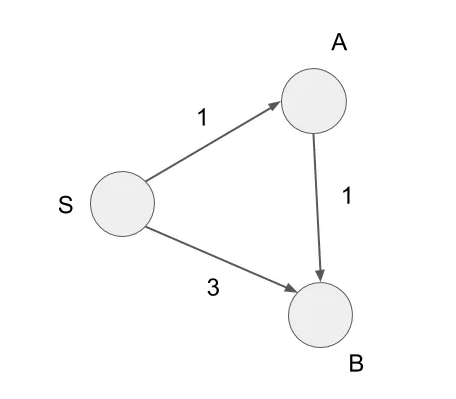
\includegraphics[width=0.6\linewidth]{images/edge_relaxation.png}    
    \caption[Caption]{Simple weighted, directed graph, used as a demonstration for edge relaxations. \footnotemark}
    \label{fig:edge_r} 
\end{figure}

\footnotetext{\url{https://towardsdatascience.com/algorithm-shortest-paths-1d8fa3f50769} [Accessed 18th March 2023]}

As an example, consider the graph in \autoref{fig:edge_r}. If we run Dijkstra's algorithm on this graph with starting vertex \emph{S}, we get distances \emph{A=1} and \emph{B=3} after the first pass. After the second pass however (exploring from vertex \emph{A}), we find an alternate path to \emph{B} (\emph{S->A->B}), the length of which is lower than our tentative distance for \emph{B} (1+1 < 3). Therefore, an \textbf{edge relaxation} is completed as the distance is updated to \emph{B=2} and the graph is fully explored.

\subsubsection{Vertex to be relaxed and vertex relaxed to.}

When looking at edge relaxations, the two vertices which the relaxed edge connects are referred to as the \emph{vertex to be relaxed} (or \emph{vertex relaxed}) and the \emph{vertex relaxed to}. More specifically, the vertex further away (in terms of shortest distance) from the starting vertex is the \emph{vertex relaxed}, while the one closer is the \emph{vertex relaxed to}. So, for the example in \autoref{fig:edge_r}, \emph{B} is the \emph{vertex relaxed} and \emph{S} is the \emph{vertex relaxed to}.

\subsection{KMP}

The \textbf{Knuth-Morris-Pratt (KMP)}\footnote{\kmpurl [Accessed: 18th March 2023]} algorithm is a string searching algorithm that efficiently finds all occurrences of a pattern string \emph{P} in a text string \emph{T}. It was developed by Donald Knuth, James H. Morris, and Vaughan Pratt in 1977. The KMP algorithm is widely used in various applications such as text editors, word processors, and compilers.

The basic idea behind the KMP algorithm is to use the information of previous matches to avoid unnecessary character comparisons in the text string. Specifically, it constructs a prefix function that computes the length of the longest proper prefix of \emph{P} which is also a suffix of each prefix of \emph{P} (stored in a \emph{border table}). This information is then used to determine the starting position of the next comparison when a mismatch occurs.



The following definitions describe important characteristics for this process of building a border table (as \emph{KMP exercises} require students to construct a border table):
\subsubsection{Border.}

A border is a non-empty proper prefix of a string that is also a suffix of that string. More formally, let \emph{s} be a string. A border of \emph{s} is a string \emph{b} that satisfies the following two conditions:
\begin{enumerate}
	\item
	\emph{b} is a proper prefix of \emph{s}, i.e., \emph{b} is not equal to \emph{s}.
	\item
	\emph{b} is also a suffix of \emph{s}, i.e., the last few characters of \emph{s} match the first few characters of \emph{b}.
\end{enumerate}
For example, the string "abab" has two borders: "a" and "ab". Both "a" and "ab" are non-empty proper prefixes of "abab" and are also suffixes of "abab".

\subsubsection{Border table.}

A border table is a data structure that stores the lengths of the borders of all prefixes of a given string. This can be implemented as an array of integers - let us call it \emph{B} - where each entry \emph{i} corresponds to the length of the longest border of the prefix of the string that ends at position \emph{i}. The first entry of the border table is always zero since the empty string has no border.

For example, consider the string "ababaca". The border table for this string would be:

\begin{table}[!h]
\begin{center}
\begin{tabular}{|c||c|c|c|c|c|c|c|}
	\hline
	i & 0 & 1 & 2 & 3 & 4 & 5 & 6 \\
	\hline
	s & a & b & a & b & a & c & a \\
	\hline
	B[i] & 0 & 0 & 1 & 2 & 3 & 0 & 1 \\ 
	\hline
\end{tabular}
\caption{\label{tab:b-table}Border table example}
\end{center}
\end{table}


In \autoref{tab:b-table}, the entry B[2] = 1 corresponds to the length of the longest border of the prefix "ab" of the string "ababaca". This border is "a", which has a length of 1. Similarly, the entry B[4] = 3 corresponds to the length of the longest border of the prefix "ababa" of the string "ababaca". This border is "aba", which has a length of 3.

\subsubsection{Overlapping border.}
An overlapping border is an informal term for referring to a border of a string where the end of the prefix border and the beginning of the suffix border overlap.

For example, the string "ababa" has a border "aba", where the last \emph{a} in the prefix border and the first \emph{a} in the suffix border refer to the same character in the string. This border would therefore be considered an overlapping border. Note that the overlapping element can be a single character or a longer substring.


%==================================================================================================================================
\chapter{Analysis/Requirements}
\label{chap:req}

This chapter introduces the requirements which ought to be fulfilled to satisfy the aims set for the project in \autoref{chap:intro}. These requirements are formulated using the research on prior works as well as the terms and concepts defined in \autoref{chap:back}, along with my experiences as a student and my supervisor's teaching experience. As the project essentially has two different products (the program which teachers use to generate and the exercises/solutions themselves given to students), separate requirements must be designed accordingly.
\section{User personas}

The two distinct users are highlighted by the following user personas.

\subsection{Teacher}

Lisa is a lecturer of computing science at the University of Glasgow. She is teaching a third-year undergraduate algorithmics course, which prominently features graph and string search algorithms (such as \emph{Dijkstra} and \emph{KMP}). From years of experience having taught this course, Lisa has noticed an increased amount of student collusion during class tests which have been held online since the start of the COVID-19 pandemic. To address this, she is seeking a feasible solution which lets her provide each student with a class test comprised of unique examples of exercises. As upholding academic integrity is her main priority, these exercises must be uniform in difficulty but also different enough so that collusion is avoided. From a practical standpoint, she cannot design this many papers by hand, as the course has over 150 students, therefore exercises must be automatically generated in an easily distributable format. To save even more time, Lisa would prefer to have automatically generated step-by-step solutions as well, aiding the marking process and also helping students recognise their mistakes. In terms of the generation process, she wants a simple user interface which allows her to have some level of input not only to choose which exercises to generate for and how many examples but also to control the difficulty of each exercise as she desires.

\subsection{Student}

John is a third-year computing science student at the University of Glasgow and is attending Lisa's algorithmics course. He is informed that the course is looking to experiment with automatically generated exercises and solutions. While he is open to the idea, he feels strongly about certain features that the system needs to have in order to be feasible. First of all, he believes that the generated exercise must be visually clear so that they are not unnecessarily more difficult to solve than handwritten ones. In a similar vein, John feels that the exercises should be similar both visually and in content to in-class exercises he has experience with so that they apply well to the course and do not cause any added confusion. Furthermore, he requires clear instructions to further ensure a good experience. In terms of the generated solutions, John thinks that if each step is explained in detail, he would be very interested in using them for revision purposes.

\section{Program requirements}

In this section, the requirements for a functional and usable automated exercise generation program are outlined. The MoSCoW method\footnote{\url{https://en.wikipedia.org/wiki/MoSCoW_method} [Accessed 18th March 2023]} is used to categorise each requirement based on importance, as highlighted below.

\subsubsection{Must have.}

These requirements encapsulate the minimum viable product, thus the program becomes unusable if any of these are not delivered.
\begin{itemize}
	\item
	\emph{Produce exercises for the two chosen algorithms (\textbf{Dijkstra} and \textbf{KMP})}: The program must be able to fulfil its main goal, which is to generate examples of exercises for each 		selected algorithm, which are output in some format. Without this feature, the application would have no real use case. 
	\item
	\emph{Ensure uniform difficulty between generated examples}: There must be algorithms in place to address the trade-off between collusion and similarity in difficulty, as highlighted in \autoref{sec:aim}. One way of achieving this is through the template-based approach as seen being successfully used by \cite{Sad12}, to organise each type of exercise by its unique characteristics, which can in turn be controlled to manipulate difficulty. If this issue is not addressed (random generation), the generated exercise would not uphold academic integrity. Each exercise's characteristics should be controllable by the user.
	\item
	\emph{Generate at least 50 separate examples of exercises in one execution}: The program must be able to generate exercises for an entire cohort of students, which may be around 50 to 300 or more students. Therefore, at the bare minimum, 50 samples of exercises need to be able to be produced from a given set of input constraints. This number should be able to be controlled by the user.
	\item
	\emph{Generate unique exercises}: Generated exercises must all be unique, to avoid collusion between students. Fortunately, due to the high number of input variables involved in our approach which can be manipulated, identical exercises are highly unlikely because of entropy\footnote{\url{https://en.wikipedia.org/wiki/Entropy_(information_theory)} [Accessed 18th March 2023]}. Thus, this requirement does not need to be enforced explicitly.
	\item
	\emph{Generate exercises in a reasonable time frame}: If the generation process takes hours to complete, the main purpose of not hand-designing each unique exercise is lost. Therefore, the process of exercise generation must be relatively time efficient. 
\end{itemize}

\subsubsection{Should have.}
The features in this section increase the usability of the program significantly but are not strictly required for a functional product.
\begin{itemize}
	\item
	\emph{Basic user interface}: The application should at least have a command line based user interface, where teachers can choose various inputs for their desired generations (number of exercises, difficulty, etc.). Without this feature, users would be required to edit the source code or use command line arguments, both of which cannot be expected from people with limited technical experience. 
	\item
	\emph{Automatic answer key}: Even though the minimum viable product handles generating the exercises themselves,  it does not provide the corresponding solutions to these problems, causing the marking process to be drastically prolonged. Having the program generate these solutions would therefore save a lot of time for teachers. Additionally, users should be able to choose whether or not they require these answer keys to speed up execution times in the cases that they do not.
	\item
	\emph{Generate LaTeX files}: The program should output each generating exercise and solution as its own LaTeX so that these can be easily distributed to students as a compiled PDF file. Having the exercises only within the program itself would make the distribution process very long as they would have to be output individually.
\end{itemize}
\subsubsection{Could have.}
The requirements in this section are in no way essential to the functionality of the program, however, they do improve user experience.
\begin{itemize}
	\item
	\emph{Simple visual user interface}: While command line interfaces offer unmatched simplicity, they can often be difficult to use, slow and confusing. To solve this, a simple \emph{JavaFX}   user interface could be implemented, allowing users to give inputs more easily.
	\item
	\emph{Step-by-step solutions}: Building on the requirement about solution generation in the previous section, the program could also generate step-by-step instructions on how to solve a given exercise. These would provide students with the tools to self-mark their solutions while clarifying any confusion that may occur without having to consult a teacher. Similarly to automatic answer key generation, users should be given the option to opt-out, speeding up the runtime.
	\item
	\emph{Generate PDF files}: The generated LaTeX files cannot be viewed directly as they must first be compiled to PDF, PNG or other formats. This process of compiling a PDF file could be done by the program itself through an API, further automating generation and distribution.
\end{itemize}
\subsubsection{Will not have.}
Since this project has a strict time limit, some requirements which \emph{Could Have} been implemented but are prioritised lower can be found in this section. Note that these features could be seen as a suitable starting point for future work in this field.
\begin{itemize}
	\item
	\emph{Automatic exercise generation for more than two algorithms}: The obvious way to further develop the program would be by implementing new generation algorithms. This process is made streamlined by the fact that the application was made with scalability in mind, so newly designed algorithms can easily be added in the future.
	\item
	\emph{Refined user interface}: As the program evolves with more generation algorithms being added, there comes a point where a simple user interface no longer suffices. At this stage, a system-wide visual overhaul may be considered, perhaps including switching to a web-based platform, to be more accessible to teachers worldwide. 
	\item
	\emph{Automatic feedback generation}: The third major area of automated exercise generation is automatic \emph{feedback} generation as highlighted by \cite{Sad12}. This process involves an entirely different approach to anything tackled in this project, as the inputs change to students' answers, which are automatically reviewed and given feedback. Therefore, this area could be the subject of an entirely new project.
\end{itemize}

\section{Generated exercise and solution requirements}

In this section, requirements for the generated exercises and solutions can be found, once again categorised by the MoSCoW method. Many characteristics are shared between Dijkstra and KMP which comprise the \emph{Shared Requirements} section, however, they both have unique features as well, which are listed separately.

\subsection{Shared requirements}
\subsubsection{Must have.}
\begin{itemize}
	\item
	\emph{Valid exercises}: The exercises which are generated must have a valid solution, otherwise they would cause a lot of ambiguity if they were to be used in an examination setting. For example, a graph generated for a Dijkstra exercise must be undirected, weighted and connected. Furthermore, there cannot exist any errors such as duplicate edges or weights between two vertices.
\end{itemize}
\subsubsection{Should have.}
\begin{itemize}
	\item
	\emph{Correct solutions}: For both standard and step-by-step solutions, they should give correct answers to their corresponding exercises. Without this, solutions become redundant.
	\item
	\emph{Clear instructions}: Exercises should have clear instructions for what they are asking of the students, using language based on existing examples of exercises. This is done to ensure that there is no added confusion as a result of automatic generation.
	\item
	\emph{Step description}: In step-by-step solutions, it is often not enough to show the intermediate output of the algorithm, as these can sometimes be confusing. To address this, the solutions should include a short description of what is being done at each step, making it easier for students to follow along. 
	\item
	\emph{Familiar and accessible visuals}: The visuals of all exercises and solutions should look similar to past exams or in-class examples. This is a necessity for ensuring that no extra burden is being put on students compared to traditional examinations. Furthermore, mildly visually impaired students (colour-blind, etc.) should not have any issues viewing the generated exercises and solutions.
\end{itemize}
\subsection{Dijkstra requirements}
\label{sec:dijkr}
\subsubsection{Must have.}
\begin{itemize}
	\item
	\emph{Labelled vertices}: Vertices in the generated graph must be labelled, as these will be used as a reference in the answer key as well as in students' solutions. 
	\item
	\emph{Edges with weight labels}: As Dijkstra's algorithm requires a weighted graph, the edges must have weight labels for the shortest paths to be calculated.
\end{itemize}
\subsubsection{Should have.}
\begin{itemize}
	\item
	\emph{Answers provided in a table}: As the exercise is asking for the shortest path and length from a chosen vertex to all other vertices, these can be displayed and tracked in a table where each row corresponds to a vertex and the three columns are: vertex label, shortest path and length of the path. This also works well in step-by-step solutions, as the table can be updated with each round of the algorithm.
\end{itemize}
\subsubsection{Could have.}
\begin{itemize}
	\item
	\emph{Edge and vertex highlights}: In step-by-step solutions, references could be made to the original graph by highlighting certain edges and/or vertices based on what Dijkstra's algorithm is working on in each pass. This would help students visualise how the algorithm works, without having to back to the graph and figuring out for themselves.
	\item
	\emph{Adjacency matrix}: In examples of graphs with a larger number of vertices and edges, edge weights can sometimes be difficult to read. To solve this issue, the graph's adjacency matrix could be provided with each exercise, offering another point of reference for students. This is a great accessibility feature, as it supports people who visualise matrices more easily than graphs.
	\item
	\emph{Highlight edge relaxations}: Since students often struggle with finding and handling edge relaxations \cite{} when using Dijkstra's algorithm, they could be highlighted in the solution table of step-by-step answer keys. This can be done by showing which two paths (with distances) are being compared and whether or not this comparison results in an edge relaxation.
\end{itemize}
\subsubsection{Will not have.}
\begin{itemize}
	\item
	\emph{Custom edge weight placement}: As mentioned earlier, bigger graphs tend to be harder to read due to overlapping edge weights. This may be solved using a custom algorithm which ensures that they are always visible, however, this proved to be slightly too time-consuming for this project.
\end{itemize}
\subsection{KMP requirements}
\subsubsection{Must have.}
\begin{itemize}
	\item
	\emph{String with borders}: The one feature that is truly essential for building a border table in KMP is the string itself, which must be built up in a way that corresponds to user inputs.
\end{itemize}
\subsubsection{Should have.}
\begin{itemize}
	\item
	\emph{Border table in solutions}: In the case of solution generation, the border table can be updated as the algorithm traverses each character in the string, updating the values as borders are found. This helps students visualise how to arrive at the final border table, which is found at the last step.
\end{itemize}
\subsubsection{Could have.}
\begin{itemize}
	\item
	\emph{Border table highlights}: To further aid with the visualisation of results, the string itself and the border table can be highlighted to represent the progression of the algorithm. This is especially useful when trying to find a specific step of the algorithm, which can now be done at a glance.
	\item
	\emph{Border found highlight}: If a border is ever found, it could also be highlighted (with different visuals to the previous requirement), to show which exact substrings the algorithm is referring to when updating the values of border length. This feature is most useful when dealing with overlapping borders, as these can often be harder to find.
 \end{itemize}
\subsubsection{Will not have.}
\begin{itemize}
	\item
	\emph{String search}: Since KMP is a string search algorithm, it may be odd to see that the exercises generated do not involve searching for a string. This in fact would require a separate generation algorithm, as it deals with an entirely new type of exercise.
\end{itemize}
\section{Changes to requirements}

As this project subscribes to an agile development process\footnote{\url{https://en.wikipedia.org/wiki/Agile_software_development} [Accessed 18th March 2023]}, there were some changes made to requirements, based on supervisor feedback, changing priorities, and time constraints.

Many of these changes can be found in the \textbf{Will Not Have} sections, as most of these requirements started as \textbf{Could Have}'s but were unable to be completed due to time constraints. For instance, early on during the design phase of the project, generating for more than two algorithms was considered. This idea was dismissed, since it was decided that refining the existing generation algorithms and adding further features to them would be more beneficial for highlighting the benefits of automatic exercise generation, as opposed to repetitively designing a new algorithm. 

Towards the end of the development cycle, a decision had to be made between implementing a simple user interface for the program or developing step-by-step solution generation, as there was only enough time left for one of them. Following discussions with my supervisor, it was decided that the increased functionality of having step-by-step solutions outweighs the usability advantages of having a dedicated user interface. Furthermore, it was noted that the program does not have enough features to warrant a more sophisticated UI, therefore would only be required once more generation algorithms are implemented. As the decision was made, the requirements were updated accordingly.


%==================================================================================================================================
\chapter{General Design}
\label{chap:des}

This chapter discusses the key design decisions made throughout the project, which aim to create a product that satisfies the requirements drawn up in \autoref{chap:req}. As part of these decisions, the final design will be highlighted along with certain alternatives and why they were rejected.

\section{Template Design}
\label{sec:td}

It became apparent quite early on in the project that ensuring uniform difficulty across exercises is one of the greatest challenges of automated exercise generation. This issue can be handled via the \emph{template-based approach} as used successfully in the past. \citet{Hoz21} suggest that for examples with pre-existing exam questions, they can be searched for syntactical characteristics, which are to be kept constant to ensure similar workloads for students (some of these characteristics would be altered to adjust the difficulty). This is quite helpful for our project, as there are quite a few past-paper questions to analyse for CompSci4009 and CompSci2026. \citet{Sad12} sport a similar idea, where specific exercises are given templates which highlight their common features while referencing their variables as parameters or "holes". What both of these papers have in common is that exercises need to be deconstructed into fixed and varying parts to ensure similar difficulty.

As per the aforementioned ideas, the template-based approach was used to design parameters (some of which will act as user inputs) from existing examples of exercises (\autoref{chap:ex_ex}) as follows.

\subsection{Dijkstra}
\label{sec:tdd}

When designing a weighted graph, the three main components we must consider are

\begin{enumerate}
	\item
 	The number of \emph{vertices}.
	\item
	The number of \emph{edges}.
	\item
	The values of edge \emph{weights}.
\end{enumerate}

While we could just take these three as our template parameters, this would result in very little variation between samples, as the only randomisation possible would be to change up the order of the vertices and edges. To go a step further, we must consider the unique characteristic of Dijkstra's algorithm, the number of \emph{edge relaxations}. Since we wish to control the difficulty of each exercise, this number must be kept uniform for all samples. From here follows that the number of \emph{edges} does not need to be a parameter because it can be derived from the number of \emph{edge relaxations}. In a similar vein, the values of edge \emph{weights} are also redundant as they can be derived from the number of \emph{vertices} (the more \emph{vertices} the higher \emph{weight} values are needed to avoid collisions). This is desirable, as we want to have as few user inputs as possible, to eliminate illegal values and general confusion. Therefore, the template parameters (user inputs) for Dijkstra are as follows:

\subsubsection{Number of vertices (User input).}
\label{sec:nov}

This is the most straightforward way of manipulating exercise difficulty, since the more \emph{vertices} a graph has, the more time it will take to compute its shortest distances using Dijkstra's algorithm. Therefore, this value must be kept constant for all exercises. 

In terms of the accepted range, it is technically possible to generate for any positive integer, however, visualising graphs with more than 20 vertices becomes challenging.

\subsubsection{Number of edge relaxations (User input).}
\label{sec:ernum}

To control the exercise difficulty for Dijkstra's algorithm specifically, the number of \emph{edge relaxations} must also be kept uniform. This is because graphs with the same number of \emph{vertices} may require significantly different amounts of effort to solve for Dijkstra depending on their \emph{edge relaxations}. 


\begin{figure}
    \centering
    \begin{subfigure}[b]{0.49\textwidth}
        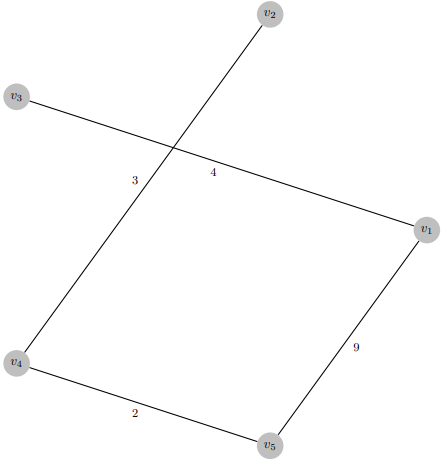
\includegraphics[width=\textwidth]{images/0relax.png}
        \caption{Graph with 5 vertices and 0 edge relaxations from \emph{v1}.}
        \label{fig:0rel}
    \end{subfigure}
    \begin{subfigure}[b]{0.49\textwidth}
        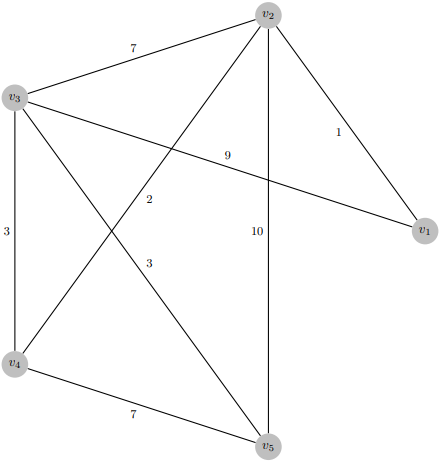
\includegraphics[width=\textwidth]{images/4relax.png}
        \caption{Graph with 5 vertices and 4 edge relaxations from \emph{v1}.}
        \label{fig:4rel}
    \end{subfigure}   
    \caption{Two random weighted graphs with the same number of vertices (5) but different numbers of edge relaxations (0, 4) from \emph{v1}. Shown side by side to demonstrate how edge relaxations control the number of edges. }\label{fig:relax_compare}
\end{figure}

As shown by \autoref{fig:relax_compare}, the number of \emph{edges} of a graph (4 and 8) is directly correlated to the number of \emph{edge relaxations} (0 and 4 starting from \emph{v1}) when looking at two weighted graphs with the same number of \emph{vertices}. This is because a single \emph{edge relaxation} requires three edges, shown by taking the example of \emph{v1}, \emph{v2}, and \emph{v3} from \autoref{fig:4rel}, with \emph{v1} being the starting vertex:
\begin{enumerate}
	\item
	Edge \emph{a} from \emph{v1} to \emph{v2}.
	\item
	Edge \emph{b} from \emph{v1} to \emph{v3}.
	\item
	Edge \emph{c} connecting \emph{v2} to \emph{v3}, where \emph{len(a+c) < len(b)}, causing an edge relaxation.
\end{enumerate}

Thus, adding more \emph{edge relaxations} results in having more \emph{edges}. This means that exercises with more \emph{edge relaxations} are inherently more difficult to solve, as more comparisons are required to be made due to the higher number of \emph{edges}, let alone considering the effort needed to keep updating the shortest distances. 

The minimum number of edge relaxations is 0, while the maximum \emph{r} for a graph with a number of vertices \emph{v} and \emph{n=v-2} is:

\begin{equation}
	\label{eq:relax}
	r = \frac{n (n + 1)}{2}
\end{equation}

This follows from the fact that (if inserting in order) after the second vertex (graphs with 0, 1 and 2 vertices cannot have any edge relaxations, hence the \emph{n=v-2}), each additional vertex provides the possibility of one more edge relaxation than its predecessor (third vertex can have one by connecting it to the first, fourth vertex can have two by connecting to the first and second, etc.). This corresponds to the series of the sum of natural numbers\footnote{\sumurl [Accessed 18th March 2023]}, with \autoref{eq:relax}.

From these two parameters, other characteristics of Dijkstra's algorithm can be acquired in the following way:

\subsubsection{Number of edges.}
\label{sec:noe}

As previously described, the \emph{number of edges} is directly controlled by the \emph{number of edge relaxations} parameter, therefore it gets adjusted automatically by the generation algorithm, so there is no need for it to be user input. Furthermore, having the \emph{number of edges} as user input along with the \emph{number of edge relaxations} would cause many input errors, as graphs with more edge relaxations require more edges by design. 

\subsubsection{Edge weights.}

This leaves the challenge of what values to assign to each edge weight. While this could also be a user input (maximum weight, distribution, etc.), we want to keep the generated exercises as simple arithmetically as possible (keep the student's efforts focused on Dijkstra's algorithm) and want to minimise the number of input variables, therefore this can also be handled internally. In essence, there is no hard limit to the values of the weights but they are weakly correlated to the number of vertices, as a larger graph requires higher weight values to avoid overlapping when it comes to generating edge relaxations. Furthermore, edge weights have certain limitations to satisfy the number of edge relaxations required, therefore they must be assigned by the algorithm. This process is further explained when exploring the Dijkstra exercise generation algorithm in \autoref{sec:dgen}. 

\subsection{KMP}

To arrive at a string from which a border table can be constructed, there are countless user inputs (template parameters) which may be considered. However, we want to optimise this number to minimise the moving parts accessible by users (avoid input errors) while still providing teachers with ample control over the difficulties of the generated exercises. Keeping this in mind, the following parameters were chosen as user inputs from reviewing existing KMP exercises (\autoref{fig:kmp_example_exercise}).

\subsubsection{String size (User input).}

The most straightforward characteristic of a string in KMP is its length. This must be controlled, as the longer the input string, the more effort it will take students to construct its border table. Having this be a fixed input does not cause any issues, as the content of the string can still be randomised to give ample variation between generated samples.

This input must be a natural number, however, larger numbers may be more difficult to visualise.

\subsubsection{Longest border size (User input).}

Since it is very complex to control the entire distribution of borders which make up a string, the next best thing is to focus on the border which takes the most effort for students to find, being the longest one. This is because tracking down longer borders means more chances for mistakes. Taking the longest border as a user input lets teachers manipulate the overall difficulty, as the algorithm will ensure that all other borders are shorter than it.

The range for the largest border is at the minimum \emph{1} and for non-overlapping borders at the maximum $floor(\frac{l-1}{2})$ where \emph{l} is the length of the string. This follows from the fact that a border cannot overlap itself, so it must be shorter than half of the string. In the case of an overlapping border, its maximum is more complex, so it is explained in \autoref{sec:ob} in detail. More on overlapping borders is discussed in the upcoming section.

\subsubsection{Overlapping or Non-overlapping longest border (User input).}

Tracking the largest border size as well as whether or not the largest border is overlapping becomes quite difficult as it can lead to input errors (ie. inputs of largest border size $b > floor(\frac{l-1}{2})$ along with non-overlapping border). These errors must be handled by the generation algorithm. It is necessary to have the \emph{overlapping} boolean as user input, however, as it significantly alters exercise difficulty. Even though there is no functional difference between overlapping and non-overlapping borders for the KMP algorithm, how \emph{humans} search for borders (usually separately traversing from the beginning and end of a given substring) makes handling overlapping borders much more challenging. The root cause of this issue deals with complex human psychology, which is outside the scope of this project (\autoref{sec:future_work}).

As previously mentioned, the input variable for overlapping border is a boolean.

The following characteristic could have been considered as user input, however, was omitted due to reasons explained below.

\subsubsection{Alphabet.}
\label{sec:alphabet}

The last aspect of a KMP border problem which has not yet been addressed is the \emph{alphabet} (selection of characters) from which characters are pulled to build the final string. It is desirable to have a limited \emph{alphabet} (instead of just generating from all Latin letters or characters), to ensure that the random selection of characters forms borders instead of getting lost in entropy.
 
The alphabet is not required to be included in the list of user inputs, since there exists a standard alphabet for border table problems in algorithmics. This alphabet usually consists of a random choice of three characters from the characters \{A,C,G,U,T\}, which originally reference nucleobases in RNA and DNA decomposition (adenine, cytosine, guanine, uracil and thymine)\footnote{\url{https://en.wikipedia.org/wiki/Nucleobase} [Accessed 18th March 2023]}.

\section{User Interface Design}

Initially, a simple command line user interface was developed, as it was a quick and easy way of testing the functionality of the generation algorithms. Later on in the development cycle, it was decided that the entire process of designing and implementing a more sophisticated UI would not be the most efficient use of time, as it may even hurt the usability of the program if poorly designed. Therefore, the command line interface was improved to be more user-friendly instead. A screenshot of the final user interface can be found in \autoref{chap:user_interface}

The advantages of a command line UI lie in its simplicity, meaning that it is easy to use regardless of experience and relatively fast. However, this simplicity comes at the price of functionality. This is because command lines only deal with strings as inputs and outputs, sometimes causing confusion when it comes to what users are expected to input. Therefore, the main aim of a successful command line interface design is to minimise this confusion as much as possible by formulating questions/prompts with straightforward answers, as well as providing ample error checking.

The following section introduces the prompts in the order in which they appear in the program's user interface, along with reasons for their specific wording and how corresponding user inputs are error checked.
\begin{itemize}
	\item
	\emph{Would you like to generate solutions? (y/n)}: This is an overarching question about solution generation, such that if the answer is \emph{n}, no solutions will be generated whatsoever. A guide to the expected input is included at the end of the prompt \emph{(y/n)}, to clarify to users that the input the program is looking for is either the character \emph{y} (for yes) or \emph{n} (for no). This is reinforced by the code, as the interface keeps prompting the user to try again until one of the two desired characters is entered.
	\item
	\emph{Would you like to generate step-by-step solutions? (y/n)}: This question only appears if \emph{y} was answered to the previous question, and is more focused, meaning that if the answer to it is \emph{y}, it will generate step-by-step solutions, and if it is \emph{n}, it will generate the final solutions only. Once again an answer guide is included, along with input error checking.
	\item
	\emph{Would you like to render to PDF? (y/n)}: This question is quite straightforward, with the input of \emph{y} resulting in both .tex and .pdf generations, while \emph{n} will limit the output to .tex only. The same guide and error checking is present as the first two questions.
	\item
	\emph{Which algorithm/s would you like to generate for? (Can choose multiple, enter to confirm) \\ Available algorithms: [(2) KMP, (1) Dijkstra]}: This is the most complex question, as it provides the option for multiple inputs. Users can either enter the name of their desired algorithm or the corresponding number as shown in the guide, to select the algorithms for which they want to generate for. An additional tip is included to prompt users that they can enter multiple algorithms and that they must press enter again to submit their choices. To aid with keeping track of which algorithms have already been selected (increasingly important as more algorithms are implemented), the following prompt appears after each input is submitted: \emph{Currently selected algorithms:(2) KMP, (1) Dijkstra}. 
\end{itemize}

After these general questions, the UI displays specific questions belonging to each selected algorithm. These questions correspond to the user inputs highlighted in \autoref{sec:td} and all include guides and error checking.

\section{Technologies}

To make implementation as trouble-free as possible, the correct development tools had to be chosen, ensuring that they can facilitate the program as designed. This section discusses how and why certain technologies were chosen.

Since automated exercise generation only became an area of focus for researchers with the rise of the COVID-19 pandemic, there does not yet exist a universally standard technology for implementation. For instance, \citet{Hoz21} used mostly Haskell and some Python, while \citet {Esh22} used Java entirely, with \citet{Kot19} implementing a web-based approach with PHP and JavaScript. This gave us a lot of freedom to choose how we were going to implement our solution. 

\subsection{Java}

Since this project is dealing with generating for different \emph{types} of exercises, it is natural to consider an object-oriented programming language for its implementation. This way, each selected exercise can be represented as a class, allowing specific examples of exercises to be instances of their corresponding exercise class. Out of the object-oriented languages, I have the most experience with Java, therefore this will be chosen of this project. Java also has excellent frameworks for user interfaces (ie. JavaFX), in case a more sophisticated user experience is required in the future.

\subsection{LaTeX}

In terms of the actual exercises and solutions generated, there is no alternative to LaTeX. Outputting .tex files of the generated exercises gives teachers the freedom to choose which format they wish to distribute them in, as well as the option to modify or combine them as they wish.
 
%==============================================================================================================

\chapter{Dijkstra design}

\section{Generation algorithm}
\label{sec:dgen}

The Dijkstra exercise generation algorithm consists of the following three main steps and essentially works by reversing Dijkstra's algorithm (starting with the shortest lengths/paths and building the graph from there):

\begin{enumerate}
	\item
	Generate the lengths of the shortest paths to each vertex from the starting vertex. (\autoref{sec:shortestpathdesign})
	\item
	Insert vertices into the graph by connecting them based on their shortest distances. (\autoref{sec:vi})
	\item
	Insert additional edges for edge relaxations, creating the final graph. (\autoref{sec:er})
\end{enumerate}

The upcoming sections describe each step in detail, including how they work and why certain design decisions were made. 

\subsection{Shortest path length generation}
\label{sec:shortestpathdesign}
\begin{enumerate}[i]
	\item
	\emph{Set an upper bound for the lengths of the shortest paths.} It is necessary to choose an appropriate value, since if too low, the number of shortest length variations decreases drastically, and if too high, generated exercises may become arithmetically difficult. While it could have been included as a user input, the maximum distance for this project is $v*3$, where $v$ is the number of vertices in the graph. Since path lengths are randomly chosen from unique natural numbers below this limit, it translates to an average difference of $3$ between each shortest path, which is scalable and arithmetically feasible.

	\item
	\emph{Generate shortest distances.} As mentioned before, these are randomly chosen (apart from the starting vertex \emph{v1}, which always has a distance of $0$) unique natural numbers below the specified limit. It is most important to note that these values are unique. This limitation is required since graphs containing vertices with matching shortest lengths are significantly more difficult to solve than ones without (confusion about which edge to explore next). If the generated values were non-unique, some graphs would display this quality while others would not, breaking the principal aim of the project. Furthermore, later parts of the generation algorithm would have to be redesigned to handle these cases (further explored in \autoref{sec:future_work}), thus including the \emph{unique} limitation is much more convenient, while maintaining the academic integrity of the generated exercises.
\end{enumerate}

At the end of this process, we are left with randomly generated shortest lengths for each vertex, which are then used to start building the graph.

\subsection{Vertex insertion}
\label{sec:vi}

Throughout the vertex insertion process, vertices are considered one by one in increasing order of shortest distance. This process can be broken down into two main parts:

\begin{enumerate}[i]
	\item
	\emph{Insert the first two vertices}. The starting (root) vertex is inserted first, so it is simply added to an empty graph. Then, the following vertex is inserted through an edge to the starting vertex with the weight of its shortest distance, since there does not exist any other vertex to connect to. These two vertices are also added to an empty n-ary tree (with the starting vertex as the root), as this will help with the insertion of the remaining vertices. This is possible because we are currently building a graph of shortest paths only (the graph is acyclic), so it can be represented as an n-ary tree.
	\item
	\emph{Insert the remaining vertices.} Adding the remaining vertices becomes much more complex. This is because the generated graph must be able to satisfy the required number of edge relaxations, which may not be possible with random insertion. As an example, if every vertex is by chance directly connected to the starting vertex via their shortest distances, no matter how many edge relaxations are needed, none will be achieved as all the shortest paths are found during the first pass of Dijkstra's algorithm. Therefore vertices must be inserted \emph{dynamically}, keeping track of edge relaxations during the process.
\end{enumerate}

The number of edge relaxations a single inserted vertex can provide is directly correlated to the number of edges which make up its shortest path to the starting vertex. This is equivalent to the level at which it exists in the n-ary tree representation of the graph. More specifically, the number of edge relaxations from a single inserted vertex $er = L-1$, where $L$ is its level in the tree (starting vertex is at level $0$). This follows from the definition in \autoref{sec:ernum}, claiming that each vertex can have an additional edge with its grandparent and up (in the tree), which form edge relaxations. 

For example, a vertex inserted at $L=4$ can provide $3$ edge relaxations by having edges of certain weights to its ancestors in levels $2$, $1$ and $0$. The reason for using an n-ary tree instead of just the number of edges in vertices' shortest paths, is that there might be separate paths to each level in the tree, each of which can be used to satisfy a certain number of desired edge relaxations, thus there must exist a variable which groups them, being the tree node level.

The naive approach would be to simply insert each vertex at the deepest level in the tree, resulting in a graph which allows for the maximum number of edge relaxations possible, meaning that the desired number of edge relaxations can be satisfied no matter what. The issue with this is that the graphs created end up having very uniform answers for Dijkstra's algorithm, as all the shortest paths being able to be found just by following the edges with the lowest weights.

Instead, vertices are to be inserted \emph{dynamically}, ensuring that the graph being built can facilitate the number of edge relaxations required while providing diverse answers. To achieve this, some characteristics of the graph must be tracked, as defined below.

\begin{itemize}
	\item
	The number of possible relaxations ($pr$) refers to the maximum number of edge relaxations which is achievable for the current graph, given that the remaining vertices are inserted in a way which facilitates this (at the maximum level each time). This variable is instantiated to the maximum number of edge relaxations for a graph with the corresponding number of vertices (\autoref{sec:ernum}) and decreases if a vertex is inserted in a way that does not maximise the number of edge relaxations. 
	\item
	Disparity ($d = p - r$) is to be interpreted as the number of possible relaxations the graph can afford to lose (where $r$ is the number of relaxations required). This variable is used to check whether or not the algorithm can afford to not maximise the number of edge relaxations in the current vertex, by checking the worst-case scenario for the upcoming vertex.
	\item
	The maximum number of relaxations from one vertex ($mr$) refers to the number of edge relaxations that the last vertex will provide if all vertices from this point are inserted in a way in which the number of edge relaxations in maximised (deepest level in tree). Initially, this variable is $v-2$, where $v$ is the number of vertices in the graph, as per \autoref{sec:ernum}. This value is important because $pr$ decreases by this much if a vertex is not inserted at the deepest level.
\end{itemize}

Given these definitions, the algorithm for \emph{ii} is the following:

\begin{enumerate}[I]
	\item
	\emph{Choose an appropriate level at which the vertex can be added in a way that the desired number of edge relaxations is achievable.} The main limitation that has to be considered is the fact that $pr$ is decreased by $mr$ each time a vertex is not inserted at the deepest possible level. This follows from the definition of $pr$. Thus, we are left with two cases.

	\begin{description}
		\item[$d < mr$:]
		The chosen level must be the deepest in the tree, as otherwise, the graph would lose $mr$ possible relaxations, which it cannot afford according to its $d$. 
		\item[$d >= mr$:]
		The algorithm has a lot more freedom to choose which level to insert the vertex. This is because the graph can afford to lose $mr$ possible relaxations, thus the current vertex can be inserted at any existing level (or one higher if inserted at the deepest level), which is handled via a random choice.
	\end{description} 

	\item
	\emph{Connect new vertex.} Randomly choose an existing vertex from the group of vertices at the given level, which will be referred to as the \emph{start} vertex. The new vertex is then joined to the graph via an edge to the \emph{start} vertex, setting the weight to be (shortest distance to new vertex - shortest distance to start vertex), which will always be positive as vertices are inserted in order of increasing \emph{shortest distance}.  Additionally, the new vertex is also added to the tree as a child of the start vertex, to match the tree to the graph. At the same time, vertices which can be relaxed are stored in a separate data structure, along with the closest vertex they can be relaxed to (two generations above them).

	\item
	\emph{Update variables.} If the insertion happened at the deepest level of the tree, a new deepest level is formed but there are otherwise no changes to the variables. In any other case, $pr$ is decreased by $mr$ (since the graph is losing out on $mr$ relaxations by not inserting at the deepest point) followed by $mr$ being decreased by one (since the deepest possible level is also being decreased by one). 
\end{enumerate}

At the end of the entire process of vertex insertion, we are left with an acyclic graph containing all the vertices. Running Dijkstra's algorithm on this current graph would give the correct answers, however, the edges which facilitate edge relaxations are still yet to be added, which happens in the final part of the generation algorithm.

\subsection{Edge relaxations}
\label{sec:er}

To have Dijkstra's algorithm perform the required number of edge relaxations, the same number of additional edges are to be inserted into the graph, therefore the following process is executed this many times. There exist certain constraints that apply to these edges, which are also explored in this section.

\begin{figure}
    \centering
    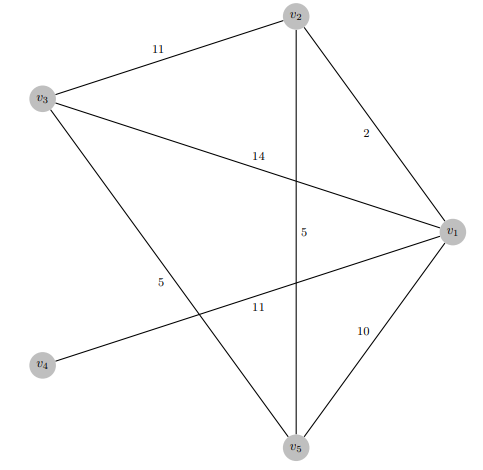
\includegraphics[width=0.6\linewidth]{images/relaxWeight.png}    

    \caption{Weighted graph with 5 vertices and 3 edge relaxations.}
    \label{fig:relaxWeight} 
\end{figure}

\begin{enumerate}[i]
	\item
	\emph{Select the vertex to be relaxed (start) and the vertex relaxed to (end).} This is done through a random selection from the list of vertices which can be relaxed (as built in \autoref{sec:vi}), while also retrieving the vertex to which we are relaxing. \emph{End} is a vertex that exists along the shortest path to \emph{start}, where adding a new edge between them (of weight larger than the path between them) creates a new edge relaxation. It is important to note that \emph{end} is initially the vertex two levels above \emph{start}, since the relaxed edge weights must increase as \emph{end} gets moved up until reaching the root.

	\item
	\emph{Calculate the weight of the new relaxed edge.} As previously mentioned, this weight must increase as \emph{end} moves up the tree, so we must first retrieve the weight which was assigned the previous time the vertex was relaxed. If this does not exist (first relaxation), the new weight must simply be larger than the length of the path between \emph{start} and \emph{end}. If it does exist, the new weight must be greater than the sum of
\begin{itemize}
	\item
	The distance between the current \emph{end} and the previous \emph{end}.
	\item
	And the previous weight. 
\end{itemize}
This is because these two values represent the length of the subsequent path explored by Dijkstra's algorithm to \emph{start}, which would not count as an edge relaxation if longer than the new relaxed edge. In either case, the increase in weight is constituted by a random integer between 1 and 3, optimising arithmetic difficulty and exercise variance.

As an example, consider \autoref{fig:relaxWeight}, where $v3$ is first relaxed to $v2$ (two before it) and then to $v1$ (root). During the first relaxation, the new edge weight ($11$) must be greater than the length of the path between \emph{start} ($v3$) and \emph{end} ($v2$), which it is, since $11 > (12 - 2 = 10)$ ($12$ being the shortest distance to $v3$ (2+5+5) and $2$ being the shortest distance to $v2$. For the second relaxation, the new edge weight ($14$) must now be greater than $(11 + (2-0)) = 13$ (shortest distance to $v1$ is $0$), which is also satisfied.

\item
\emph{Use \textbf{start}, \textbf{end} and \textbf{weight} to insert a new edge, facilitating a new relaxation.} Additionally, data structures storing previous weights and distances are updated. The \emph{end} vertex belonging to the current \emph{start} must be moved one step closer to the root. The only complexity here is checking if \emph{end} already is the root, in which case \emph{start} has no more relaxations and can be ignored in subsequent passes. Otherwise, the vertex to which it is to be relaxed to is updated.
\end{enumerate}

In the end, the algorithm outputs a graph which has the required number of vertices ($v$) and edge relaxations ($r$) for Dijkstra's algorithm. The graph also has $(v-1) + r$ ($v-1$ for initial connection of vertices and $r$ for relaxed edges) edges, reinforcing the claim that the number of edges is directly correlated to the user inputs in \autoref{sec:noe}.

\section{Exercise and solution design}


Similarly to how templates are designed for the chosen exercises in \autoref{sec:td}, templates for the visualisation of exercises and their corresponding solutions must also be formulated as per the requirements in \autoref{sec:dijkr}. Many ideas for the execution of this task are inspired by existing examples of exercises and solutions (\autoref{chap:ex_ex}) while ensuring that the visuals are scalable (readable for small and large inputs). Note that only step-by-step solutions are analysed when it comes to solution design, as "simple" solutions always match the outcome at which the last step arrives.

\subsection{Exercise layout}
\label{sec:dijkstraExerciseDesign}

The Dijkstra exercise task description comes from \autoref{fig:dijkstra_example_exercise}, as it perfectly outlines what students are expected to do, and has been tested in real-world examinations. A clarifying clause is included afterwards, informing students that the values of edge weights appear just off the centre points of each edge. This is to help with visualisations of larger graphs, where identifying which weight belongs to which edge can sometimes be difficult.

Another feature which helps with the scalability of generated graphs is the included adjacency matrix. The adjacency matrix acts as a last resort (since it is always readable) when some edge weights are completely obscured due to having a very large graph with many edges. 

The greatest challenge with displaying a graph comes from deciding where to place each vertex. This is a unique issue to automatic generation, since custom vertex placement (as done by hand) is not a viable option, especially as graphs get larger. The approach taken for handling vertex placement is inspired by the example exercise  \autoref{fig:dijkstra_example_exercise}, which places each vertex in a circle, with equal space between them. This is generalised by starting with \emph{v1} at \emph{0 \textdegree} (right of the circle) and adding each consecutive vertex at $p+\frac{360 }{v}$\textdegree where $v$ is the number of vertices in the graph and $p$ is the angle of the previous vertex until all the vertices are displayed. The result is a placement of vertices where they all sit even spaced on the circumference of a circle, making the graph highly scalable (at least until vertex markers physically start overlapping).

\subsection{Solution layout}

An instance of a Dijkstra exercise solution consists of the following three parts, which update at each step of the algorithm:

\begin{enumerate}
	\item
	Table showing the current shortest path to each vertex and their lengths.
	\item
	Graph from exercise highlighted to show the progression of the algorithm.
	\item
	Short description of what happened in the current step and what is going to happen in the following step.
\end{enumerate}

The solution table is very similar to the example solution in \autoref{fig:dijkstra_example_solution}, however, it does have some unique features. Since it represents the state of Dijkstra's algorithm as it explores each vertex, early on during execution there will be vertices which have not yet been found, which are represented as a path of $null$ and length $\infty$. These values are then updated continuously, displaying each comparison and its result (ie. $11 = min(\infty, 2+9)$). This also applies to edge relaxations, which are specifically in bold to highlight them (this is indicated to students at the end of each step).

The main graph is also altered at each step. Vertices are highlighted to showcase which of them have been visited and highlighted edges show which new edges are considered in the current pass of the algorithm. These make it easy to visualise how Dijkstra's algorithm explores the entire graph.

The short description at the end of each step highlights the current and the next vertices to be explored. This may be helpful for colour-blind or visually impaired students, who find it easier to follow text rather than the colours on the graph.

%===============================================================================================================

\chapter{KMP Design}

\section{Generation algorithm}
\label{sec:kgen}

The KMP exercise generation algorithm consists of two main steps:
\begin{enumerate}
	\item
	Generate the largest border. (\autoref{sec:ob} and \autoref{sec:nob})
	\item
	Fill out the rest of the string. (\autoref{sec:remainder})
\end{enumerate}

The process of largest border generation differs drastically depending on if it is overlapping or not, so these are addressed in separate sections.

\subsection{Overlapping border generation}
\label{sec:ob}

To generate an overlapping border, it must be deconstructed into smaller parts which are more manageable. Every overlapping border must consist of the same beginning and end substring, since the end of the prefix border has to match the beginning of the suffix border, forming the overlap (thus this substring is referred to as the \emph{overlap} or $o$). 

The remaining part of the border (substring between the two \emph{overlaps}) can be randomised from the alphabet, as it does not affect the overlapping process, and is called the \emph{middle} (or $m$). Considering these two substrings, the structure of an overlapping border is $o+m+o$.

 As an example, the overlapping border "aba" from the string "ababa" has \emph{overlap} "a" (at the beginning and end) and \emph{middle} "b" (could be any other string). Considering both prefix and suffix borders joined, the structure becomes $o+m+o+m+o$ ("$a+b+a+b+a$").

Following the above definitions, the overlapping border generation algorithm consists of the following steps:

\begin{enumerate}[i]
	\item
	\emph{Calculate the length of the overlap.} \textbf{If} the length of the \emph{largest border (lb)} is longer than half of the entire \emph{string (s)} size, the length of the \emph{overlap (ol)} must be
	\begin{description}
		\item[(ol > lb - (s / 2)):]
		This refers to the amount by which the longest border overhangs half of the entire string, meaning that the overlap must be higher to physically fit the combination of prefix and suffix borders in the final string.
		\item[(ol < (lb / 2) - 1):] Since a border is made up of two instances of \emph{overlap} (and one \emph{middle} giving \emph{o+m+o}), the length of one \emph{overlap} must be smaller than half of a border (-1 to at least have one character for \emph{middle}), otherwise the two \emph{overlaps} would physically not fit in the required longest border size.
	\end{description}
\textbf{Otherwise}, the minimum value is simply $1$. 

	\item
	 \emph{Calculate the maximum length of an overlapping border.} Taking the maximum overlap length (the shortest the prefix + suffix can be), if the length of $o+m+o+m+o$ is greater than the required length of the string, then the given border length is too long (cannot be fit into the string). This holds because if the border required is too long, the \emph{overlap} length must increase to try and fit the borders, however, if the overlap gets too large, the generated borders will once again be too long as well (the prefix and suffix have three instances of \emph{overlap}).

\item
\emph{Insert border.} The length of the \emph{middle} is $m = b - 2 * o$ where $b$ is the length of the longest border (as follows from $b = 2 * o + m$). From here, $m$ and $o$ are randomly generated from the selected alphabet, and inserted at the beginning of the string under the pattern $o+m+o+m+o$, forming the largest overlapping border. Note that this border will always be at the beginning of the string since the prefix and suffix must physically overlap.
\end{enumerate}

\subsection{Non-overlapping border generation}
\label{sec:nob}

Generating and inserting a non-overlapping border is much more straightforward. 
\begin{enumerate}[i]
	\item
	\emph{Define the starting position for the suffix} (the prefix is always at the beginning). This is to be after the prefix border (so they do not overlap) and 'largest border length' spaces before the end of the string (so it fits) and is chosen randomly. 
	\item
	\emph{Generate the random border.} Given the starting position, a random border can be generated from the selected alphabet and trivially inserted at the beginning of the string (prefix) and chosen starting position (suffix). 
\end{enumerate}

\subsection{Remainder of string}
\label{sec:remainder}

The last step is to fill in the remainder of the string while handling edge cases.

\begin{enumerate}[i]
	\item
	\emph{Handle the longest border edge case.}  If the "random" character following the prefix border matches the "random" character following the suffix border, we have an issue, as this would form a border that is longer than required. To handle this, the algorithm first inserts a random character after the prefix and then inserts a character which is different after the suffix.

	\item
	\emph{Populate the remaining unfilled spaces with random characters from the alphabet.} With this approach, there is a possibility that the longest border appears more than two times (prefix and suffix). This in itself would not be a problem, since the longest border found in the string would still be the required length. The issue comes from when the subsequent character from this new largest border matches the subsequent character from the prefix border, creating a longer than desired largest border.

	\item
	\emph{Handle "multiple longest border" edge case}. Search for the largest border in the temporary final string. Once an instance of the largest border is found, if it is not the original prefix or suffix border, the first character of it is changed, so that there is no longer an unintended match with the longest border.
\end{enumerate}

At the end of the process, the program outputs a string of the required length, which contains a largest border of the desired length and type.

\pagebreak

\section{Exercise and solution design}

\subsection{Exercise layout}
\label{sec:KMPExerciseDesign}

The design for KMP exercises is less complex than Dijkstra, since a string is inherently less visual than a graph, thus needing fewer adjustments. The task description comes from a combination of example exercises  (\autoref{fig:kmp_example_exercise}), which importantly specify that students need not use the KMP algorithm, they must simply construct the border table required for KMP. The alphabet of the generated string is also displayed, to provide context.

\subsection{Solution layout}
\label{sec:KMPSolutionDesign}

The step-by-step solutions are similar to the exercises in their simplicity, as they merely show how the border table gets updated as the generated string is being traversed (\autoref{fig:kmp_example_solution}).

However there are some additional features which help students with understanding how border tables are built. Firstly, the substring which is currently being checked is highlighted in both the string itself (red) and the border table (bold). This aids with the ease of following the progress the algorithm is making. Additionally, whenever a border is found, it is pointed out in two different ways. It is displayed in bold in the string, and it is also mentioned in words (along with the length of the border) at the end of the step. This text says "No border found." in any other case.

%==================================================================================================================================
\chapter{Implementation}
\label{chap:imp}

The Java implementation\footnote{\url{https://github.com/zsojtory1/automated-exercise-generation/tree/main/src}} of the program utilises an object-oriented design. Both chosen exercises (\textbf{Dijkstra} and \textbf{KMP}) have custom classes, which describe important characteristics of each exercise and handle generation. Additionally, the \textbf{Visualiser} class includes the implementation of the user interface along with the LaTeX and pdf generations.

\section{Dijkstra}

\subsection{Constructor}

Every Dijkstra exercise is generated through the constructor. This method takes the designed user inputs (int \emph{vertices} and int \emph{relaxations} from \autoref{sec:tdd}) as arguments and starts by doing error checking on them. If any input is not within the legal range, Java throws an IllegalArgumentException with an error message, otherwise, fields are instantiated as with any other constructor. The two most important methods called by the constructor are \emph{generateDistances} (computes the output for Dijkstra's algorithm) and \emph{generateGraph} (builds the graph itself), details of which are explained in the following sections.

\subsection{Method \texttt{generateDistances}}

This method randomly generates the shortest distances to each vertex in the graph, as per the maximum distance defined in \autoref{sec:shortestpathdesign}. As with all future mentions of randomly selected integers, this is handled by \emph{ThreadLocalRandom.current().nextInt}. This result is stored in a LinkedHashMap, mapping from each vertex (represented as unique integers from $0$ to $v-1$) to their respective distance (unique integer). 

The reason a LinkedHashMap is used as opposed to a regular HashMap is that during graph generation we wish to traverse vertices based on increasing shortest distance, thus our data structure must be able to be sorted (regular HashMaps have no order so they cannot be used). This sort is done after the distances are generated, by calling the \emph{sortMap} method. This method sorts by converting the entries in the original map to a list of entries and then utilising the Java Collections package to call \emph{Collections.sort}. Since this function cannot handle sorting between entries by default, it is fed a custom comparator class (\emph{valueComparator}), which compares entries based on their values. Finally, the sorted list is converted to a new LinkedHashMap and returned.

\subsection{Method \texttt{generateGraph}}
\label{sec:generateGraph}

This method constitutes the main chunk of the program (implementation of \autoref{sec:dgen}), building a weighted graph based on the user inputs and shortest distances generated in the previous method. The returned graph is a custom object of type \textbf{WeightedGraph.Graph}. Each instance of this class contains its number of vertices (int) and two LinkedLists of lists of edges, constituting the \emph{directed} and \emph{undirected} adjacency lists of a graph. It is useful to have both, as \emph{undirected} is important for functionality, while \emph{directed} is used for visualisations. \textbf{Edge} is also a custom class, which has \emph{start} (int), \emph{end} (int) and \emph{weight} (int) attributes.

This method uses several data structures to handle the functionalities introduced in \autoref{sec:dgen}, as described below.
\begin{itemize}
	\item
	\emph{HashMap<Integer, Integer> relaxedTo} has keys of vertices which can be relaxed, mapping to the next vertex to which they should be relaxed.
	\item
	\emph{HashMap<Integer, Integer> relaxedWeight} stores the weight that was used in the vertex's previous edge relaxations so that it can be increased in the following relaxation.
	\item
	\emph{HashMap<Integer, List<Integer>> vertexToPath} maps each vertex to its shortest path to the root vertex. The path is represented as a list of vertices (integers), from the root to the given vertex.
	\item
	\emph{HashMap<Integer, Integer> prevDist} maps each vertex to the shortest distance of the vertex it was previously relaxed to, allowing further relaxations to be made.
\end{itemize}

Outside of these data structures, a custom implementation of an n-ary tree is used during the process of inserting vertices into the graph. This is handled by the \textbf{NaryTreeNode} class, which has attributes \emph{val} (\emph{int} referring to a vertex), \emph{level} (\emph{int} referring to the level in the tree at which the node exists, with the root being $0$) and \emph{children} (List<NaryTreeNode> referring to all the children of the node). 

\begin{figure}
    \centering
    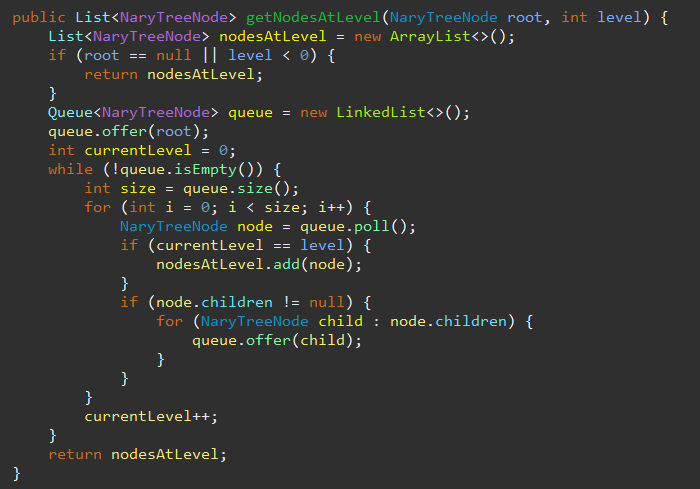
\includegraphics[width=0.7\linewidth]{images/levelTrav.png}    

    \caption{Implementation of tree traversal, retrieving all the nodes at a chosen level.}
    \label{fig:levelTrav} 
\end{figure}

Traversing through the LinkedHashMap of vertices (\emph{shortestDistance}), the closest two vertices (\emph{root} and \emph{next}) are first added to the graph and the tree. For any subsequent vertex, once a level is chosen, the tree is traversed to find all the vertices at the chosen level (as seen in \autoref{fig:levelTrav}). This method uses a queue to keep track of all the nodes, adding the children of each node to the same queue until every node is explored. At this point the queue is empty and the function terminates, returning \emph{List<NaryTreeNode> nodesAtLevel}, to which each node matching the level is added.

The list returned is randomly sampled, choosing a \emph{startNode} to attach the new vertex to, retrieving its vertex value with \emph{startNode.val}. It is important to retrieve the actual node instead of just the value since the new vertex must be added to the \emph{startNode} as a child to further build the tree.

Once the new vertex is added to the graph and the tree, it must also be added to \emph{vertexToPath}. This is done by taking the path of its parent (\emph{vertexToPath.get(start)}), adding the new vertex (\emph{path.add(entry.getKey())}) and finally inserting the path (\emph{vertexToPath.put(entry.getKey(), path)}).

After every vertex has been inserted into the graph, the \emph{vertexToPath} HashMap is traversed to build the \emph{relaxedTo} HashMap. The shortest path of each vertex is checked, and if they a greater than two, the vertex to which they are relaxed to is the one that is two before them in their path (as described in \autoref{sec:dgen}). This is done by setting \emph{listSize} to be \emph{vertexToPath.get(v).size()} and calling \emph{relaxedTo.put(v, vertexToPath.get(v).get(listSize-3))} if the condition holds.

To add an edge relaxation, a random key-value pair is taken from \emph{relaxedTo}. Then a value for the weight is generated using the algorithm in \autoref{fig:weight} (referring to \autoref{sec:er}). Here, we calculate the difference of \emph{prevDist.get(start)} (previous \emph{end}) and \emph{shortestDistance.get(end)} (current \emph{end}) to get the distance between these two vertices, while \emph{relaxedWeight.get(start)} retrieves the weight used in the vertex's previous relaxation. Once the weight is chosen, the new edge (facilitating the relaxation) can be inserted, along with updating \emph{relaxedWeight} and \emph{prevDist}.

\begin{figure}
    \centering
    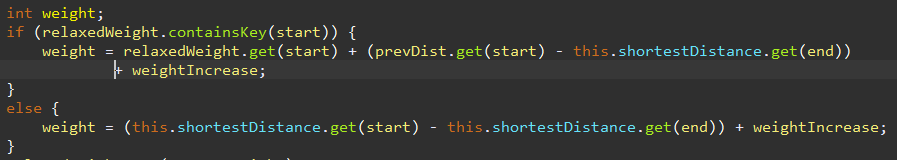
\includegraphics[width=0.99\linewidth]{images/weight.png}    

    \caption{Weight generation for edge relaxation.}
    \label{fig:weight} 
\end{figure}

\begin{figure}
    \centering
    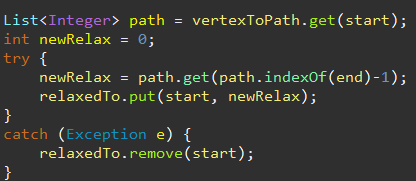
\includegraphics[width=0.5\linewidth]{images/relaxedToUpdate.png}    

    \caption{Algorithm for updating \emph{relaxedTo}.}
    \label{fig:relaxedToUpdate} 
\end{figure}

As a last step, \emph{relaxedTo} must be updated as seen in \autoref{fig:relaxedToUpdate}. The next vertex to which our selected vertex is to be relaxed to is retrieved by moving one up the shortest path (\emph{newRelax = path.get(path.indexOf(end)-1)}). This is done in a try statement since it would be null if \emph{end} was the root. In this case, the current vertex is removed from \emph{relaxedTo}, as it cannot provide any more relaxations, so it should no longer be chosen. If \emph{newRelax} is successfully retrieved, however, \emph{relaxedTo} is updated with it.

\section{KMP}

\subsection{Constructor}

The KMP constructor works much the same way as the one in Dijkstra. However, there is some added complexity when it comes to input error checking, in the case where the length of the largest border is greater than half the size of the string and is non-overlapping. When this is true, the largest border must be overlapping, as it would physically not fit otherwise, so attributes are declared accordingly. The two main methods which are called by the constructor are \emph{generateAlphabet} and \emph{generateString}, which are further explored in the following sections.

\subsection{Method \texttt{generateAlphabet}}

To generate a unique alphabet for a given exercise, the algorithm considers the base alphabet (A, C, G, U, T from \autoref{sec:alphabet}) as an array of characters (since it never changes). Then it builds the actual alphabet for the exercise by choosing three random characters from the base, while ensuring no duplicates. The result is stored in the class attribute \emph{alphabet} since it is unique for each exercise.

\subsection{Method \texttt{generateString}}

This method handles the final string generation (returned as a string), as per \autoref{sec:kgen}. Throughout the process, the following variables are updated:

\begin{itemize}
	\item
	\emph{String[] result} is an array storing the characters in the final generated string, instantiated to an empty array of the required length.
	\item
	\emph{String longestBorder} is the generated longest border.
	\item
	\emph{int borderStart} keeps track of the index of where the suffix border is to be inserted.
\end{itemize}

Since overlapping prefix and suffix borders are connected and inserted at the beginning of the string, \emph{borderStart} (initialised to $0$) is used as the index for where to insert each consecutive part of the border ($o+m+o+m+o$). Once each part is inserted, \emph{borderStart} will have the index of the value following the last character in the suffix border, which will later be used to check for duplicate borders.

The \emph{borderStart} variable is used similarly in non-overlapping borders, however, the prefix and suffix may not be adjacent in this case, so the prefix border is inserted at the beginning of the string and the \emph{borderStart} is set to a random index after it, as it is used to insert the suffix. Note, that following the insertion, \emph{borderStart} is once again pointing to the element after the end of the suffix border.

\begin{figure}
    \centering
    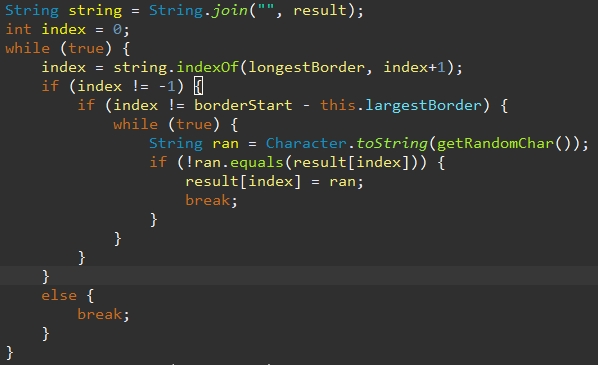
\includegraphics[width=0.7\linewidth]{images/borderSearch.png}    

    \caption{Code searching for and removing duplicate longest borders.}
    \label{fig:borderSearch} 
\end{figure}

Once the strings are completed, they must be checked for accidental generations of the longest border, which is handled as seen in \autoref{fig:borderSearch}. First, \emph{String.join} is used to convert the array of characters \emph{result} to a string. Then \emph{index = string.indexOf(longestBorder, index+1)} searches for the first appearance of the border. The second argument of \emph{indexOf} specifies the start of the search and since this equates to $0+1$ in the first pass, the prefix border will never be found (it starts at index $0$). This means that the only two conditions we must check for are:

\begin{description}
	\item[index == -1:]
 	\emph{Break} from the while loop since no more borders are found.
	\item[index != (borderStart - this.largestBorder):] 
	Border found is not the suffix, thus must be eliminated by changing its first character to something different.
\end{description}

\section{Visualiser}

This class acts as the main driver for the program, as it handles the user interface and the final generated output files. Running the program \emph{jar} file will launch the main method of this class, which calls several visualisation methods to handle the user's requests. Examples of the final visualisations can be found in \autoref{chap:visuals}.

\subsection{Method \texttt{main}}

The first thing the main method does is create new directories, in which files will be placed (separate for exercises, solution, tex and pdf) using \emph{File.mkdirs}. Then, these directories are emptied (from previously generated exercises) by calling \emph{FileUtils.cleanDirectory}, \emph{FileUtils} being a class from the \emph{Java commons io} package.

Then, a \emph{Scanner} object is used to handle user inputs. These inputs are error checked through infinite while loops (re-prompting users), which only terminate once inputs are given in the required format. Throughout this process, users are given guidance in the command line in the form of \emph{System.out.println} messages.

The most difficult user input to handle is the selection of which algorithm/s to generate for. The final implementation uses the \emph{HashMap<String, Boolean> algorithms}, mapping each algorithm to whether or not the user had selected them. Then, the user input is fed into a switch-case (each algorithm is numbered as well, so both name and number lead to the same case), changing the value of the desired algorithm to true if selected. At the same time, a \emph{StringBuilder} tracks all the algorithms which have been already chosen and is used as a reminder for the user. The default case indicates an error (prompting a retry), and the empty string is used to submit the current selections.

The actual exercises are generated by instantiating as many objects of the selected algorithm as specified by the user. Then, these objects are passed to visualisation methods (separate for exercise, solution and step-by-step solution), along with where to save them (incrementing file name) and to export to pdf or not (boolean).

As a final step, the folders where the generated files are saved are opened using \emph{Desktop.getDesktop().open}.

\subsection{Visualisation methods}

\begin{figure}
    \centering
    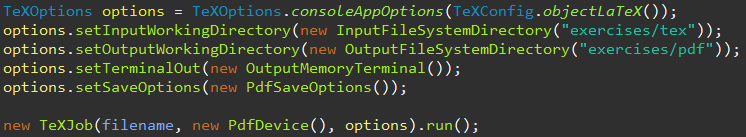
\includegraphics[width=0.9\linewidth]{images/pdf.png}    

    \caption{API calls for rendering a .tex as a .pdf file.}
    \label{fig:pdf} 
\end{figure}

These methods work by writing properly formatted .tex files for the given exercise/solution through a Java \emph{FileWriter} object. This requires some heavy string formatting in Java. Once a .tex file is generated, it may be rendered to a pdf. This is handled through an API called \emph{aspose.tex}, the code for which is highlighted in \autoref{fig:pdf}.

Each visualisation method has unique, important characteristics, as highlighted below.

\begin{itemize}
	\item
	\emph{generateGraph} handles the visualisation of Dijkstra exercises. As with all other tables, the adjacency matrix is built as a \emph{tabular}. The major challenge with this is that the size of the matrix is variable, so the number of vertices must first be checked to create the correct size \emph{tabular}. The contents of the adjacency matrix are retrieved from the undirected adjacency lists defined in \autoref{sec:generateGraph}. The graph itself is drawn using a LaTeX package called \emph{Tikz}, which enables plenty of customisations when it comes to graphs (size, shape, colour, etc.). The design of a graph is specified in \autoref{sec:dijkstraExerciseDesign}, and the actual values are retrieved from the specific exercise's directed adjacency list.
	\item
	\emph{generateGraphSolution} handles the visualisation of Dijkstra solutions. This method does not run Dijkstra's algorithm to find the solution to an exercise, as this would be time inefficient. Instead, as the shortest distances and paths of each exercise are already stored as class attributes (generation works backwards from solution), final solutions can simply be retrieved from there.
	\item
	\emph{generateFullGraphSolution}: handles the visualisation of step-by-step Dijkstra solutions. This method must use Dijkstra's algorithm since we need to display the intermediate results of the algorithm at work. This is done by taking the results from Dijkstra's algorithm after each pass and displaying the corresponding table and graph on separate pages in the .tex file.  
	\item
	\emph{generateString} handles the visualisation of KMP exercises. Not much complexity here, as it simply displays the generated string along with the question.
	\item
	\emph{generateStringSolution} handles the visualisation of KMP solutions. To do this, a custom method called \emph{constructBorderTable} is used, which returns the borders for a given KMP exercise. This is necessary because the KMP generation algorithm does not start at the solution (as opposed to Dijkstra), so it must be computed whenever it is asked for.
	\item
	\emph{generateFullStringSolution} handles the visualisation of step-by-step KMP solutions. This works similarly to the previous method. Since already established values never change in a border table (only further ones are explored), it can be calculated once at the beginning of execution. Then, the length of the border table which is displayed is incremented by one each time (filling the rest out with zeroes), to represent each step of the solution. Coloured highlights are added using the \emph{xcolor} package, as required by \autoref{sec:KMPSolutionDesign}.
\end{itemize}

%==================================================================================================================================
\chapter{Evaluation} 
\label{chap:ev}

In this chapter we discuss the methods used to evaluate the extent to which our proposed solution is successful at handling the problem proposed in \autoref{chap:intro}. The results collected from the experiments are then presented and analysed, to assess the performance of our program according to its target users.

\section{Aims}
\label{sec:evalAims}

Even though the aims of the project are highlighted in \autoref{sec:aim} (generate exercises which are non-unique, but similar in difficulty), comparing the difficulties of two exercises is not only very difficult but also quite subjective (people perceive difficulty differently and approach exercises differently). Therefore, the evaluation conducted places its focus on the following key areas, which were deemed integral to the main problem:

\begin{enumerate}
	\item
	\emph{How similar are generated exercises/solutions to pre-existing example exercises/solutions of the same type?} This applies to both form and content and helps with determining how useful automatic exercise generation can be.
	\item
	\emph{What are some of the ethical implications of automatic exercise generation?} We asked key parties involved about their personal opinions on automated exercise generation, to gather some ethical (or otherwise) concerns they may have.
	\item
	\emph{How good is the usability of the application?} 
	\item
	\emph{To what extent are controlled and uncontrolled variables handled effectively?} This mostly refers to the template design from \autoref{sec:td} and how it could be improved.
\end{enumerate}

\section{User study design}
\label{sec:exp_design}

Since this project delivers products to two separate groups of users - namely students (receive exercises and solutions) and teachers (use the program itself) - it is only appropriate to design and conduct two distinct user studies. This is important not only because they interact with different outputs, but they might also have drastically differing personal opinions about the impact of automated exercise generation on computer science education altogether. As they are both key stakeholders in this field, their ideas must be equally considered, hence the two experiments. The full user surveys can be found in \autoref{chap:user_surveys}, along with participant instructions in \autoref{chap:participant_instructions}.

\subsection{Student user study}

Students are given one example of each exercise type along with their corresponding step-by-step solutions. For Dijkstra, this is a graph with $5$ vertices and $3$ edge relaxations, and for KMP it is a string of length $13$ with a \emph{non-overlapping} longest border of size $4$. These parameters were chosen to match the size of a typical in-class example. 

To start, students are provided with a short introduction about the aims of the project and how the exercises they received were generated. Additionally, students receive detailed instructions on how to complete the user study:
\begin{enumerate}
	\item
	Open the attached Dijkstra and KMP exercises and inspect their style and format.
	\item
	Use the included step-by-step solutions to arrive at the solutions for both problems.
	\item
	Complete the survey, based on your experiences with the included exercises.
\end{enumerate}

To reduce the amount of effort required to complete the user study, students are not asked to solve the exercises, they must simply inspect them and use the included answer key to logically arrive at the solution. To further help with this process, the algorithms used to get the solutions are also included.

As the final step, participants should complete a short (4 minutes) survey, consisting of three parts:

\subsubsection{Dijkstra}

The first section includes questions about Dijkstra exercises and solutions. The questions asked are the following:

\begin{itemize}
	\item
	\emph{The Dijkstra exercises I received were similar in difficulty to exercises I have seen in class.}: Since comparing difficulty between two given exercises is very difficult, the next best approach is to compare the exercise to other examples encountered in the past. While this is not a very scientific solution (the answer will highly depend on personal experiences rather than empirical data), it is still beneficial, as we cannot forget that students are not computers, so their perception of difficulty may be more important than objective difficulty (if such a thing even exists).
	\item
	\emph{The Dijkstra exercises I received were similar in format to exercises I have seen in class.} The question refers to the style of the exercise (as defined in \autoref{sec:dijkstraExerciseDesign}), which can sometimes be just as important as the content.
	\item
	\emph{The adjacency matrices helped make the exercises more understandable.} This question aims to find out how new additions (features existing exercises do not often have) influence student perception of the exercise.
	\item
	\emph{The model solutions I received for Dijkstra exercises were easy to understand.} Another style/structure question.
	\item
	\emph{Having step-by-step solutions for Dijkstra helped with tracing the solution to the exercise.} Another new addition.
	\item
	\emph{Highlights/colours helped make each solution step be more descriptive in Dijkstra.} Style once again.
	\item
	\emph{Elaborate further about any of the answers above.} Optional long response question for any other comments.
\end{itemize}

\subsubsection{KMP}

The second section is nearly identical to the first one (excluding the questions which do not apply to KMP), just for the included KMP exercise/solution.

\subsubsection{General Questions}

The third and final section asks more open-ended and general questions, answers to which may highlight possible alternate use cases for the program.

\begin{itemize}
	\item
	\emph{Do you think receiving automatically generated exercises of the same difficulty is fair academically?}: Ethical question for examination settings.
	\item
	\emph{Do you think the use of automated exercise generation is more suitable for formative (tutorials) or summative (class test) assessments?}: Even if students may not be comfortable with receiving automatically generated exercises in examination settings, they might still be fine with using them in formative assessments.
	\item
	\emph{If you had a tool which could automatically generate exercises and step-by-step solutions, would you use it, and if so, how?} Students may have alternate use cases for the program (self-study, etc.).
	\item
	\emph{Overall thoughts and conclusions about exercises and solutions received.}: Long answer about any other comments.
\end{itemize}

Overall, this user study gathers information relating to questions $1.$ and $2.$ from \autoref{sec:evalAims}.

\subsection{Lecturer user study}

As lecturers directly interact with the program, they are given the .jar file to experiment with. Additionally, a more detailed description of the project is provided for context in a text document.

The first paragraph introduces the project by specifying the problem and the algorithms for which generation will be done. Next, the main functionality of the Java program is described, helping lecturers get a grasp of the user interface, as well as how inputs and outputs work. Lastly, brief reasons are given for the decisions behind the chosen user inputs for each generation algorithm.

For participants who do not wish to generate their exercises, five exercises and their solutions (same parameters as students) for each algorithm are also included in the user study, so that these can be inspected as references for the survey. Additionally, a screenshot of the user interface is presented so that the usability of the program can be evaluated as well.

Once lecturers are introduced to the project, they are given simple instructions for completing the user study:
\begin{enumerate}
	\item
	\textbf{Launch} the JAR file (\emph{java -jar AutomatedExerciseGenerator.jar}) and experiment with generating exercises and solutions (program will empty the destination directory with each execution). Alternatively, simply inspect the provided screenshots of the program.
	\item
	\textbf{Review} a few examples of exercises and solutions (either self-generated or the ones attached).
	\item
	\textbf{Complete} the survey.
\end{enumerate}

The survey contains the following two sections.

\subsubsection{System Usability Scale.}

The first part is a usability evaluation for the program conducted according to the \emph{System Usability Scale} (SUS). This approach is ideal, since it is an industry-standard for usability testing, especially for small sample sizes (while still delivering reliable and valid results). The results from this section can be used to deduct whether or not it would be worth it to implement a more complex user interface.

\subsubsection{General Questions.}

To keep the user study as short as possible, lecturers are not asked about specific exercises, instead focusing on more general questions as follows:

\begin{itemize}
	\item
	\emph{Do you think the use of automated exercise generation is more suitable for formative (tutorials) or summative (class test) assessments?} This question also found in the student survey, thus student and teacher perspectives can be compared in \autoref{sec:analysis}. 
	\item
	\emph{Do you think the level of input you had over the exercises generated was appropriate, and if not, how could it be improved?} Question referring to template design (\autoref{sec:td}).
	\item
	\emph{Do you think the constraints chosen for each type of exercise were appropriate? If not, do you have any suggestions for what they should be?} Similar to the previous question, asking details about specific algorithms instead of just user inputs.
	\item
	\emph{Overall thoughts and conclusions about the product.} Final comments or suggestions.
\end{itemize}

All in all, this user study addresses questions $2.$, $3.$ and $4.$ from \autoref{sec:evalAims}.

\section{Results}
\label{sec:results}

This section shares the results of the surveys described in \autoref{sec:exp_design}. Note that the user studies conducted had a limited number of participants (7 students and 4 lecturers), so the results may not accurately represent the views of the entire user base. Both user studies were conducted following the ethics form found in \autoref{chap:ethics_form}.

The student participants were all third-year computing science students to ensure that they have recent experience with the algorithms involved. The teacher participants were all lecturers of computing science possessing enough technical knowledge to use the program.

To be able to more easily compare results, each response to a question is assigned a value from $0$ to $4$ (Strongly disagree = 0, Strongly Agree = 4) to form a five-point Likert scale\footnote{\url{https://www.britannica.com/topic/Likert-Scale} [Accessed 18th March 2023]}.

Visuals of all the Likert results can be found in \autoref{sec:survey_responses}.

\subsection{Dijkstra}
\label{sec:d_results}

The results of all Dijkstra-related questions are presented in \autoref{tab:dijkstra_results}.

\begin{table}[h]
\begin{center}
\begin{tabular}{| c || c | c | c | c | c | c |}
	\hline
	Question & \ref{fig:d_similar_difficulty} & \ref{fig:d_similar_format} & \ref{fig:adjacency_matrix} & \ref{fig:d_model_solution} & \ref{fig:d_step_by_step} & \ref{fig:d_highlights} \\
	\hline
	\hline
	Mean & 3.7143 & 3.714 & 3.286 & 3.286 & 3.714 & 3.714 \\
	\hline
	Standard deviation & 0.452 & 0.452 & 0.700 & 0.452 & 0.700 & 0.452 \\
	\hline
	Median & 4 & 4 & 3 & 3 & 4 & 4 \\
	\hline
\end{tabular}
\caption{\label{tab:dijkstra_results} Results of Dijkstra questions}
\end{center}
\end{table}

\subsection{KMP}
\label{sec:k_results}

The results of all KMP related questions are presented in \autoref{tab:kmp_results}.

\begin{table}[h]
\begin{center}
\begin{tabular}{| c || c | c | c | c | c |}
	\hline
	Question & \ref{fig:k_similar_difficulty} & \ref{fig:k_similar_format} & \ref{fig:k_model_solution} & \ref{fig:k_step_by_step} & \ref{fig:k_highlights} \\
	\hline
	\hline
	Mean & 3.714 & 3.571 & 3.857 & 4.000 & 3.714 \\
	\hline
	Standard deviation & 0.452 & 0.495 & 0.345 & 0.000 & 0.452 \\
	\hline
	Median & 4 & 4 & 4 & 4 & 4 \\
	\hline
\end{tabular}
\caption{\label{tab:kmp_results} Results of KMP questions}
\end{center}
\end{table}

\subsection{Usability}
Since the usability of the system is evaluated using \emph{SUS}\footnote{\url{https://www.researchgate.net/publication/228593520_SUS_A_quick_and_dirty_usability_scale} [Accessed 18th March 2023]}, a definite score can be calculated from responses through the following method. First, take the mean result (value from $0$ to $4$ from each question across all participants. Then, for questions \autoref{fig:usability1}, \autoref{fig:usability3}, \autoref{fig:usability5}, \autoref{fig:usability7}, and \autoref{fig:usability9}, the score is simply its mean result, while for questions \autoref{fig:usability2}, \autoref{fig:usability4}, \autoref{fig:usability6} and \autoref{fig:usability8}, the score is $4$ minus its mean result (since they are worded in a way that \emph{Strongly Disagree} is the best answer). Finally, the sum of each question's scores is multiplied by $2.5$, giving the final \emph{SU} score out of $100$.

The mean results and converted scores for our evaluation are shown in \autoref{tab:sus}. From these individual scores, the final \emph{SU} score can be calculated: $(3 + 3.25 + 3.25 + 3.5 + 2.75 + 3.75 + 2.5 + 3.25 + 3.25 + 3.75) * 2.5 = 32.25 * 2.5 =$ \textbf{$80.625$}.

\begin{table}[h]
\begin{center}
\begin{tabular}{| c || c | c | c | c | c | c | c | c | c | c |}
	\hline
	Question & Q1 & Q2 & Q3 & Q4 & Q5 & Q6 & Q7 & Q8 & Q9 & Q10 \\
	\hline
	\hline
	Mean & 3 & 0.75 & 3.25 & 0.5 & 2.75 & 0.25 & 2.5 & 0.75 & 3.25 & 0.25 \\
	\hline
	Score & 3 & 3.25 & 3.25 & 3.5 & 2.75 & 3.75 & 2.5 & 3.25 & 3.25 & 3.75 \\
	\hline
\end{tabular}
\caption{\label{tab:sus}SUS means and final scores}
\end{center}
\end{table}

\subsection{General feedback}

\subsubsection{General questions.}
\label{sec:personal_questions}

The large majority of participants believed that the practice of automated exercise generation is academically fair (mean = $3.429$, s = $0.904$, median = $4$). Full results can be found in \autoref{fig:s_academic_fair}.

Most students reported that they would only be comfortable with automated exercise generation in formative assessments ($6$ formative, $0$ summative,$1$ both).  Full results can be found in \autoref{fig:s_formative_summative}.

On the other hand, lecturers generally thought that automated exercise generation is suitable for both formative and summative assessments ($2$ formative, $0$ summative, $2$ both).  Full results can be found in \autoref{fig:t_summative_formative}.

\subsubsection{Open-ended questions.}

As long-answer responses were not \emph{required} in the surveys, not many participants provided answers. The answers that were received, however, shed a light on a lot of the future work that can be explored in the context of the project (\autoref{sec:future_work}).

One student brought up the idea of vertices having the same length shortest distance in Dijkstra, which could cause problems. In hindsight, it should have been communicated to the students that this would never happen since the algorithm generates unique shortest distances for this exact reason. 

Another student praised the similar format and difficulty of questions, along with the solutions, claiming that they would use the program for self-study.

One lecturer gave some very detailed feedback on the program. They claimed that the interface was easy to use, however, they did have some suggestions for improvement. For instance, edge weights sometimes overlap for Dijkstra and the edge highlights in solutions do not communicate anything useful. Additionally, they thought that the program should not clear the target directories before generation, as this could accidentally remove files that are still needed.

On the opposite end of the spectrum, another lecturer claimed that "The text-based interface is not very easy to use.". They had further suggestions for KMP specifically, being that the number of \emph{shifts} could have been a constraint. They also commented on execution time being quite slow for generating step-by-step solutions.

\section{Analysis and discussion}
\label{sec:analysis}

In this section, we use the results of our user studies (\autoref{sec:results}) as well as personal findings to address the aims of our evaluation (\autoref{sec:evalAims}).

\subsection*{How similar are generated exercises/solutions to pre-existing example exercises/solutions of the same type?}

From the results in \autoref{sec:d_results} and \autoref{sec:k_results}, we can quite confidently conclude that students found no discernible differences between exercises/solutions that were automatically generated and hand-designed ones that they had seen previously in classes. This applies to both content and format, which is an important distinction, since it is easy to overlook visuals and focus on the seemingly more complex aspect, being the exercises themselves. Neglecting the format would not be a great idea however, as an exercise with confusing visuals is inherently more difficult to solve, which is something that we want to avoid.

One area where the visuals are not up to par at the moment is in the cases of large Dijkstra graphs. As highlighted by one of the lecturers, edge weights sometimes overlap, resulting in the situation mentioned above, so this must be addressed in the future (\autoref{sec:future_work}). 

Adjacency matrices were included with each Dijkstra exercise as a temporary solution for overlapping weight labels, however, students did not find it very helpful, as shown by the fact that it had the lowest mean score ($3.286$) out of all the questions. Since this score is above $2$, it means that while students did not find adjacency matrices to make exercises more cumbersome, they also did not find them very useful. We agree with this sentiment, since trying to solve a Dijkstra problem from an adjacency matrix only seems much more difficult (especially as the graph gets larger) than having the visual of the graph.

The reason why students did not comment on the overlapping edge weight issue is that they had a limited number of exercises available to them, with none of them suffering from this issue. Therefore, while the results are very positive, we cannot assume that our product is perfect.

For instance, even though students reported that the exercises they received are similar to something they would receive in class, there is currently not much guarantee that two examples of generated exercises (with the same parameters) are similar in difficulty, which is the main aim of the project. To address this, further user studies must be conducted (\autoref{sec:future_work}).

\subsection*{What are some of the ethical implications of automatic exercise generation?}

Even if we assume that the exercises generated are comparable in difficulty, there are still ethical issues surrounding the topic of automated exercise generation, which must be addressed.

Quite surprisingly to us, students mostly seemed to be very comfortable with the idea of automatically generated exercises as shown in \autoref{sec:personal_questions}. This is because we suspected that students would be more worried about their peers having unfair advantages in academics, which may be introduced as a result of having unique exercises. 

The responses to the subsequent question shed some light on why students were so comfortable with automated generation. An overwhelming majority prefers to have automatically generated exercises for formative assessments only, so students are confident in giving the system a try in low stake settings, such as tutorials or seminars. This makes sense because we would not want students to risk sacrificing their academic results for the sake of this new technology.

In contrast to students, teachers felt a lot more confident using automatic generation, even in summative assessments. This may be because lecturers are a lot more eager for finding efficient ways of designing new exercises (hand designing takes a lot of time), allowing them to put more energy into other aspects of their teaching.

While we started this project with the goal of reducing collusion in online examinations, from both personal experiences and user feedback, it has become clear that the tool we have created is much more useful in less crucial settings (summative or formative assessments). This is further reinforced by the student who claimed that they would use it for self-studying. Furthermore, examination boards would first have to approve the software before deployment, which is a very long and strenuous process. This shows that even though there are a lot of ethical implications involved, alternate use cases can always be found.

Another ethical issue deals with the fact that different people might approach the same exercise in different ways. Even though there are set algorithms students should follow when solving our exercises, since humans are not machines, they will often use their intuition and past experiences to find shortcuts (skip unnecessary passes of the algorithms). While some may argue that these students deserve to have an advantage for their clever thinking, the generation algorithms still assume that all humans think like computers, which may be an issue.

Even though the template-based approach used in designing these generation algorithms works very well at increasing difficulty for computers (more difficult exercises will require more passes of the exercise algorithm), this does not necessarily mean that the same effect is achieved in the case of humans, as mentioned above. Solving this issue is rather difficult, as it deals with complex human psychology (how people solve problems), which should be further investigated (\autoref{sec:future_work}).

\subsection*{How good is the usability of the application?}

According to the \emph{System Usability Scale}, a \emph{SUS} score of above $68$ is considered above average, so our score of $80.625$ indicates an interface that works well for its purpose.This should by no means suggest that the system is perfect, as a number of its flaws were highlighted by our user study and personal experiences with using it.

The worst performing question (as per \autoref{tab:sus}) is \emph{Q7}, which is \emph{I would imagine that most people would learn to use this system very quickly.}. This is most likely because launching the program requires users to interact with the command line, which people with no technology background might struggle with. While the program is mostly meant for computing science lecturers (who know how to use the command line), a quick and easy fix would be to write a script which launches the application in the command line.

While some participants thought that the interface was quite easy to use, others found it rather difficult. This along with the fact that usability will only get worse as further generation algorithms are implemented lead us to believe that a more robust user interface should be implemented, as further described in \autoref{sec:future_work}.

Another observation that was reported by a lecturer is the fact that execution time is quite slow when generating step-by-step solutions. This happens because the logic for creating these visualisations is done in Java, so a lot of repeated strings are written to the output .tex file, which is a computationally expensive process. Instead, the logic should be done in LaTeX, minimising the number of strings that must be written to the .tex file. Another benefit is that the file sizes would also be smaller.

\subsection*{To what extent are controlled and uncontrolled variables handled effectively?}

While our choices of constraints were mostly praised by participants, they did have a few suggestions about areas that we did not consider.

One lecturer proposed that the query string for KMP could have been generated by taking the number of \emph{shifts} as a constraint. This parameter would consider how many counter-clockwise shifts it would take for the string to have the same length longest border as before (essentially swapping the prefix and suffix borders), in turn controlling where the suffix border is placed within the string. This may be an important constraint to include, since strings, where the longest border is found in the beginning, may be easier to construct a border table for than strings with the longest border at the end.

A student had a different suggestion for Dijkstra, where vertices with \emph{non-unique} shortest distances should be considered. Examples of exercises where this occurs drastically increase complexity, not only in terms of solving the exercise but also the generation process, since the algorithm relies on having unique shortest distances. Therefore, we believe that it is better to keep the current approach, as the implementation would require a lot of resources for a scenario that does not happen very frequently.

%==================================================================================================================================
\chapter{Conclusion}    
\label{chap:conc}
\section{Summary}

As online examinations became the norm overnight due to the COVID-19 pandemic lockdowns, student collusions increased drastically, threatening the academic integrity of these examinations. With the solution of monitoring students at home introducing serious difficulties and ethical concerns, educators seek alternate approaches to eliminating the chance for collusion.

\emph{Automated exercise generation} is an area of computing science education which aims to address this issue by providing each student with unique exam papers, so that answers cannot be shared easily between them. This process inherently has its challenges, most importantly ensuring that each generated exercise has equal difficulty while keeping them unique. A useful addition to this method is \emph{automated solution generation}, which deals with simultaneously producing answer keys to the aforementioned exercises.

To test the effectiveness of \emph{automated exercise generation} in the field of algorithmics, we designed and implemented a program which automatically generates instances of predetermined exercises, while using certain controlled variables (parameters) to ensure uniform difficulty. The two algorithms for which this generation would be done are \emph{Dijkstra}'s algorithm and the \emph{Knuth–Morris–Pratt} algorithm since they constitute two different areas of algorithmics (graphs and strings).

The generation program was then evaluated through user studies involving both students and teachers to determine how effective our solution was at maintaining similar difficulty. Due to uncertainties arising from comparing the difficulties of exercises, the focus of the evaluation was narrowed down to the following key questions:

\begin{itemize}
	\item
	How similar are generated exercises/solutions to pre-existing example exercises/solutions of the same type?
	\item
	What are some of the ethical implications of automatic exercise generation?
	\item
	How good is the usability of the application?
	\item
	To what extent are controlled and uncontrolled variables handled effectively?
\end{itemize}

These questions were answered by getting participants to review examples of generated exercises and solutions as well as the program itself, before having them complete separate surveys for students and teachers. 

From the results of our evaluation, we find that participants are in general happy with the format of the exercises, the user interface and the constraints chosen. On the other hand, they did report that most of them would only be comfortable with introducing automated exercise generation in formative assessments. Another implication that was considered is the idea that humans approach solving exercises differently from computers, so perhaps working backwards from the chosen algorithms is not the best approach for exercise generation.

Overall, we believe that our current solution does a very good job at automated exercise generation for the two types of exercise, however, more user testing is required to ensure that our main aim of delivering exercises of similar difficulty is met.

\section{Future work}
\label{sec:future_work}

From the results of our evaluation and personal observations during development, it is apparent that there is much more work to be done not only on automated exercise generation in general but on this project specifically as well.

Firstly, there are a few steps which must be taken to legitimise our findings. Namely, we should provide formalised descriptions of the designed generation algorithms along with rigorous mathematical proofs, as well as validation for the implementation (unit tests, etc.). 

Since our study was limited by its scope, it would be beneficial to run a large-scale user study to answer the main problem proposed in the paper (uniform difficulty of exercises). This could be done by giving participants examples of exercises generated with the same parameters and asking them to decide how close in difficulty they were to each other. This process would require a large number of participants, as exercise difficulty is very ambiguous, thus a big sample size is needed to arrive at a sound conclusion. This study would truly allow us to evaluate the effectiveness of our solution.

As the motivation for this project was generating entire examination papers, it follows logically that generation algorithms for additional examples of exercises should be implemented. This is because examination papers usually consist of more than two types of exercises. Once this is achieved, an evaluation could be completed testing how entirely automated generated examinations would work. While examination boards are still far from approving automated exercise generation, conducting the aforementioned study would be the first step towards this future.

To explore the area of how humans solve exercises, a collaborative study could be done with an expert in human psychology. In the user study, participants would be asked to describe in detail how they approach solving a given exercise. This would provide us additional information (along with existing exercises and the algorithms themselves) to help design our generation templates.

Automated exercise generation relates closely to another area of research, \emph{automated grading}. This involves taking student answers as inputs and calculating their marks by comparing the inputs to the actual solution. Automated grading comes with its complexities, so it was not considered for this project, however, it should be looked at in the future, as it is the last step for completing the automated generation pipeline (exercise $\rightarrow$ solution $\rightarrow$ grade).

In terms of short-term improvements to our program, a more sophisticated UI (JavaFX perhaps) becomes more and more desirable as new generation algorithms are implemented. Additionally, the issue of overlapping edge weights must be solved through some sort of custom edge weight placing algorithm, which keeps track of the positions of existing weights, so that new labels are not placed on top. Chosen user inputs could also be re-evaluated, to perhaps include \emph{shifts} for KMP or even a list of student IDs to make assigning exercises more simple.

%==================================================================================================================================
%
% 
%==================================================================================================================================
%  APPENDICES  

\begin{appendices}
\label{chap:appendices}
\chapter{Example exercises and solutions}
\label{chap:ex_ex}

\begin{figure}[h]
    \centering
    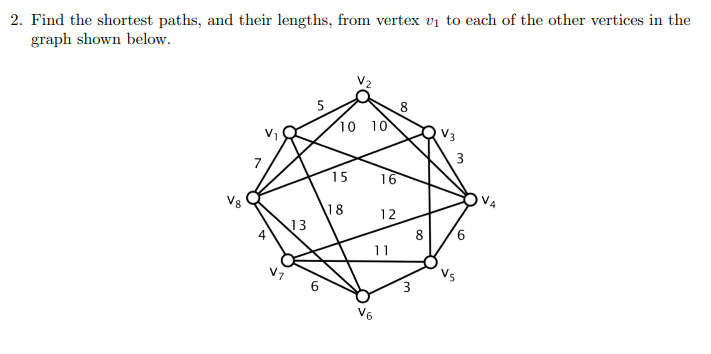
\includegraphics[width=0.9\linewidth]{images/dijkstra_example_exercise}    

    \caption{Example exercise for Dijkstra. (Dr. Oana Andrei, CompSci2026)}
    \label{fig:dijkstra_example_exercise} 
\end{figure}

\begin{figure}[h]
    \centering
    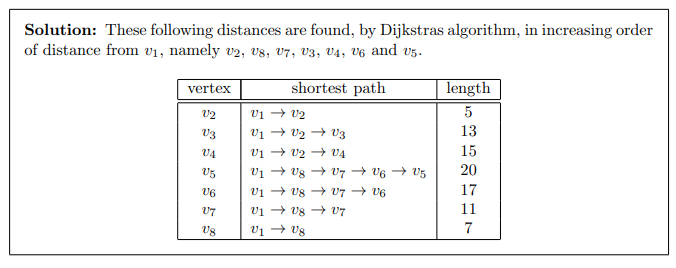
\includegraphics[width=0.9\linewidth]{images/dijkstra_example_solution}    

    \caption{Example solution for Dijkstra. (Dr. Oana Andrei, CompSci2026)}
    \label{fig:dijkstra_example_solution} 
\end{figure}

\begin{figure}[h]
    \centering
    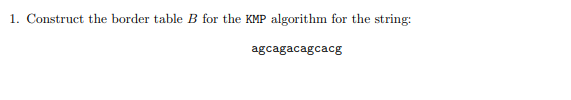
\includegraphics[width=0.9\linewidth]{images/kmp_example_exercise}    

    \caption{Example exercise for KMP. (Dr. Oana Andrei, CompSci2026)}
    \label{fig:kmp_example_exercise} 
\end{figure}

\begin{figure}[h]
    \centering
    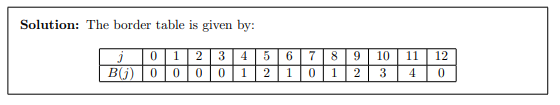
\includegraphics[width=0.9\linewidth]{images/kmp_example_solution}    

    \caption{Example solution for KMP. (Dr. Oana Andrei, CompSci2026)}
    \label{fig:kmp_example_solution} 
\end{figure}

\chapter{User Interface}
\label{chap:user_interface}

\begin{figure}[h]
    \centering
    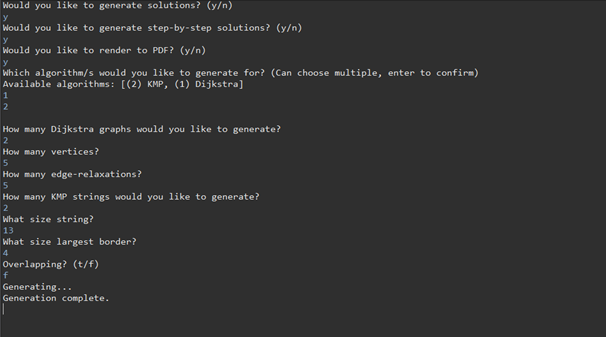
\includegraphics[width=0.99\linewidth]{images/user_interface}    

    \caption{Command line user interface.}
    \label{fig:user_interface} 
\end{figure}

\chapter{Final exercise and solution visuals}
\label{chap:visuals}

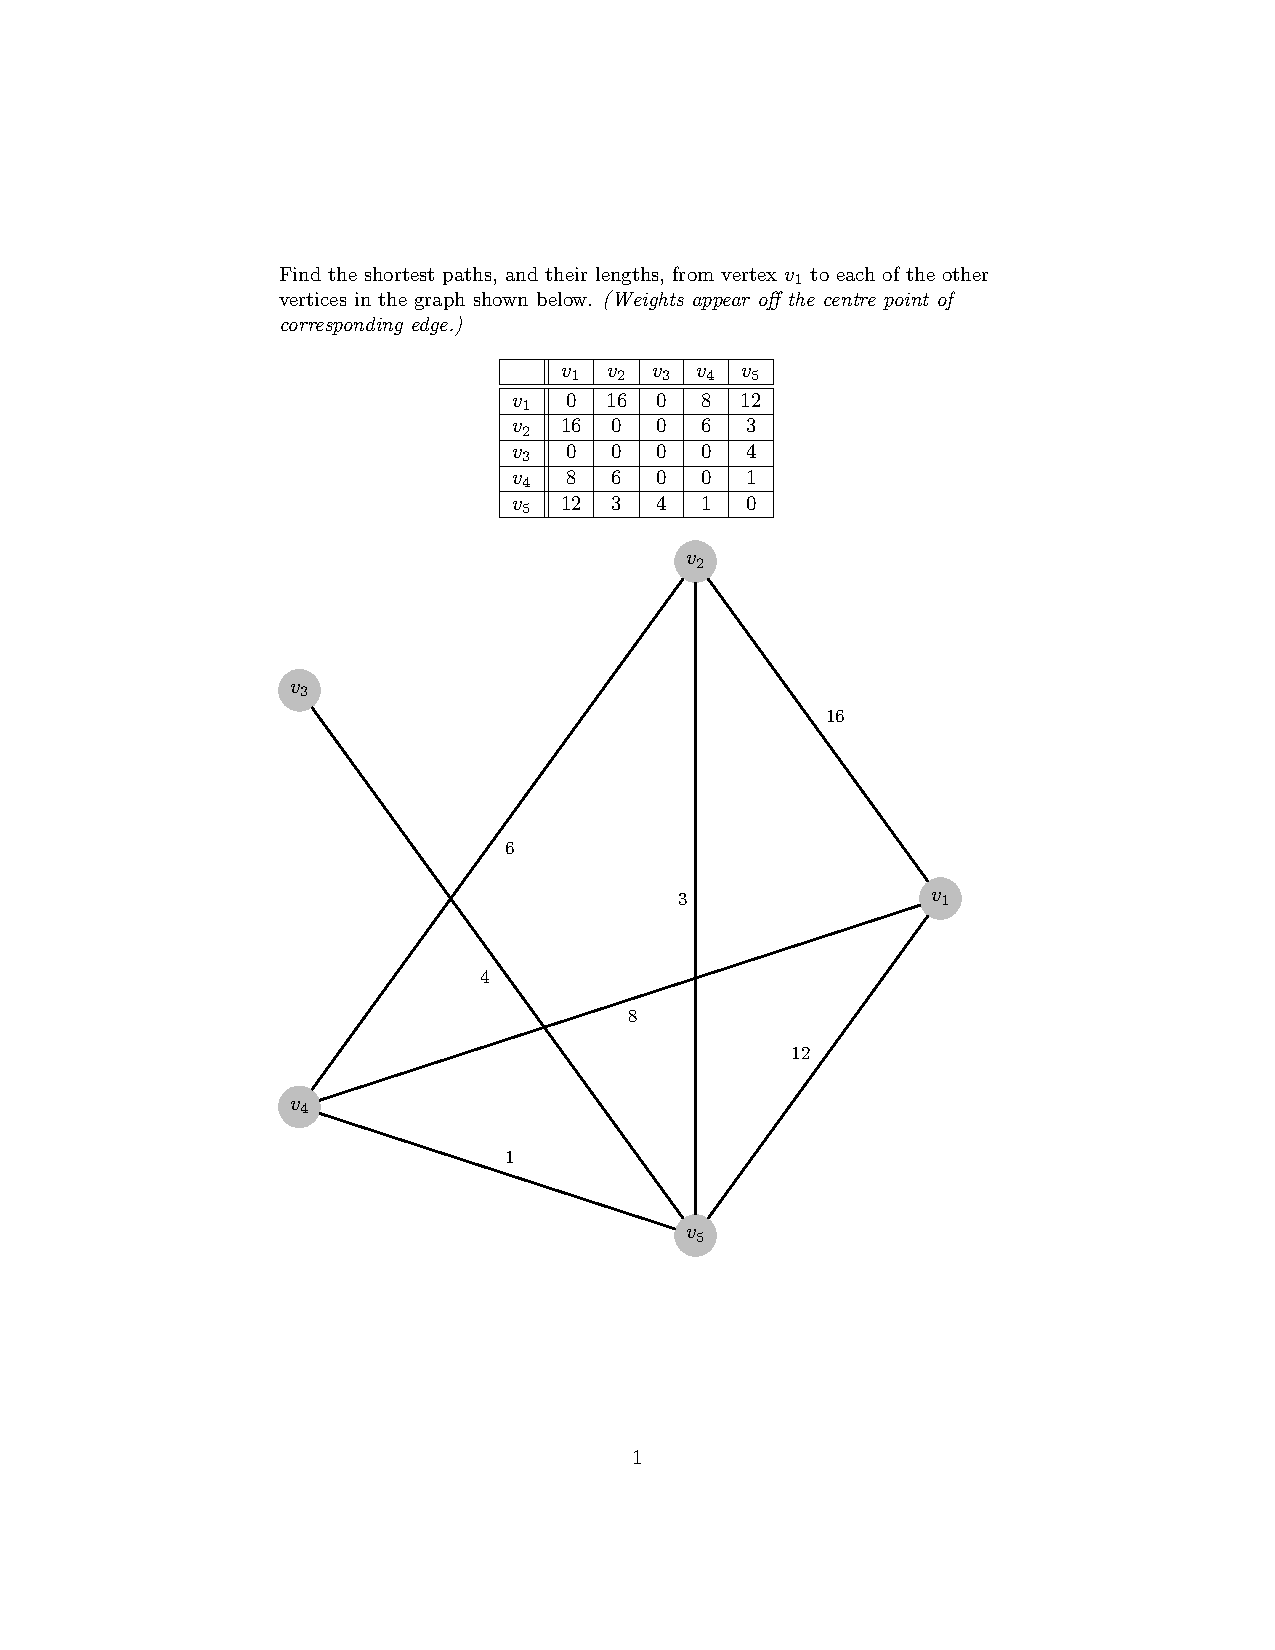
\includepdf[pages=-]{images/dijkstra1.pdf}
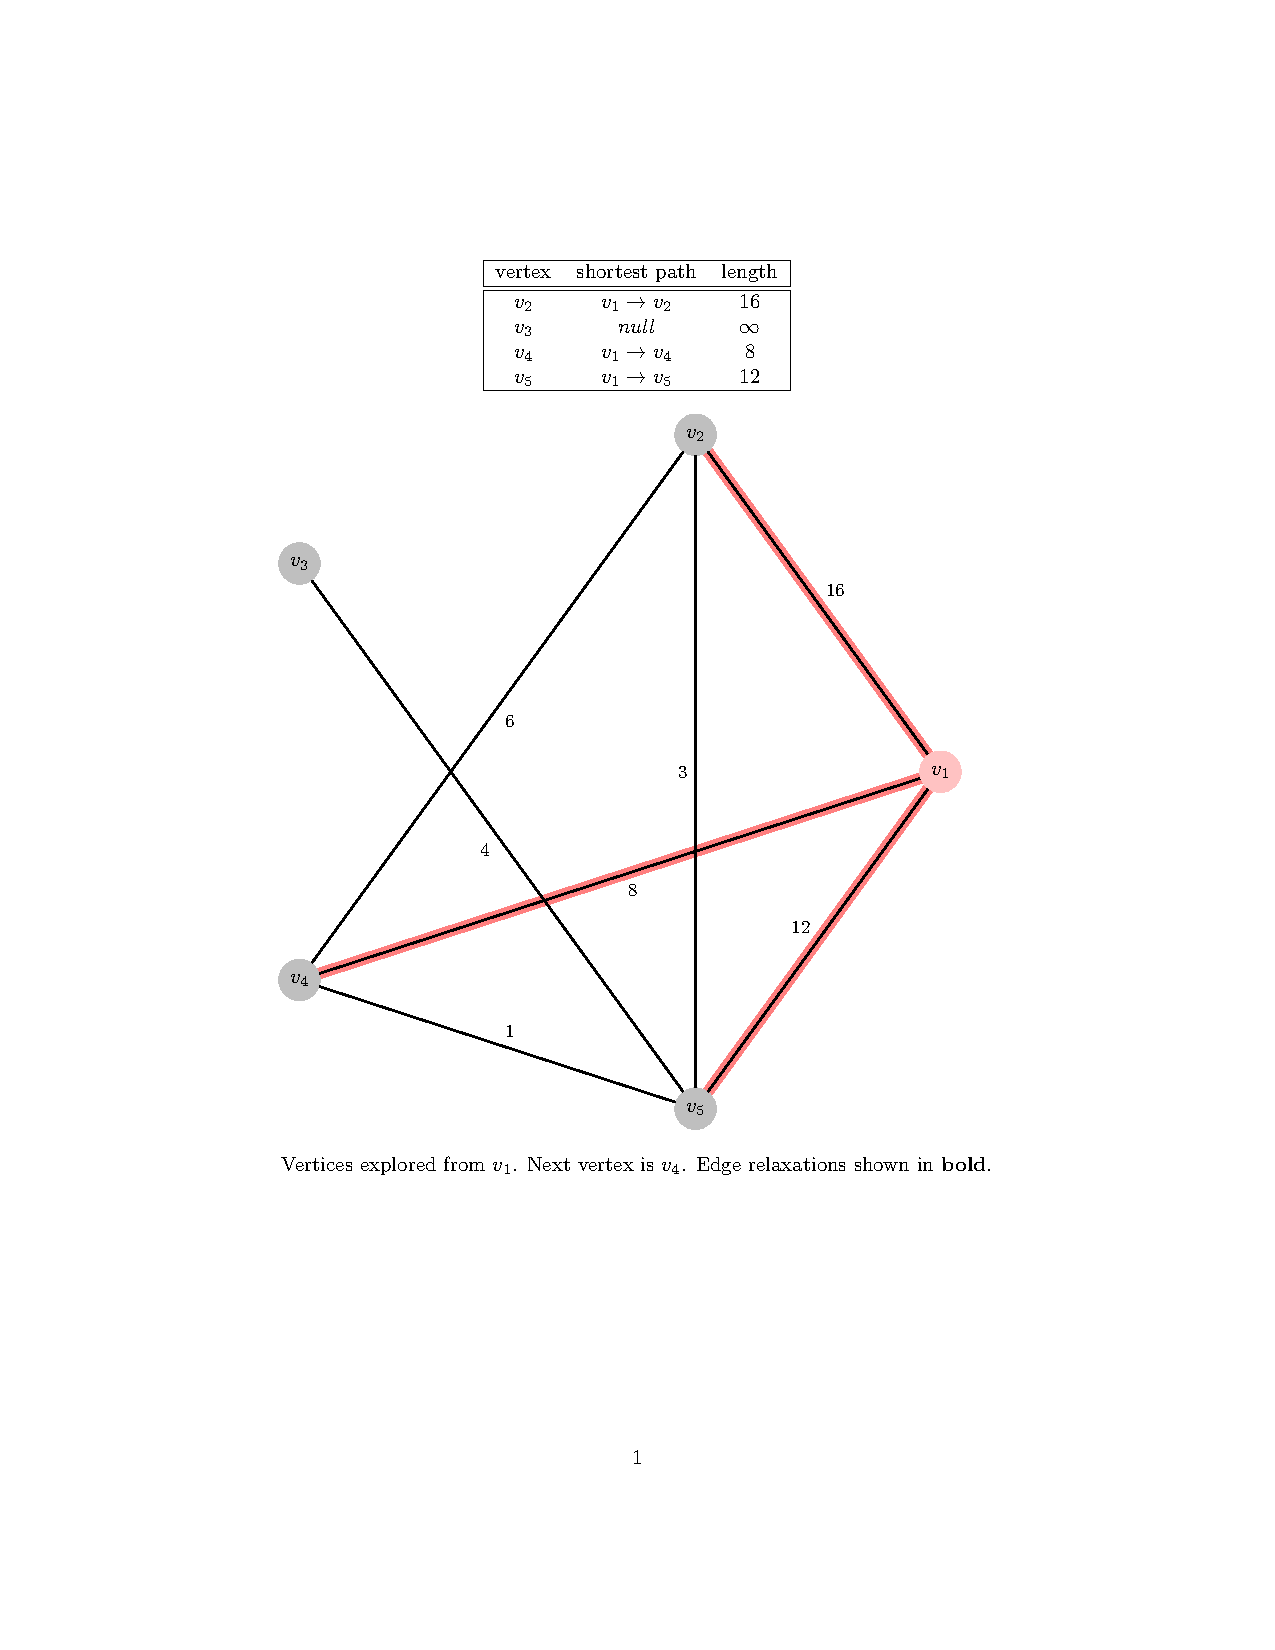
\includepdf[pages=-]{images/dijkstra_answer1.pdf}

\includepdf[pages=-]{images/kmp1.pdf}
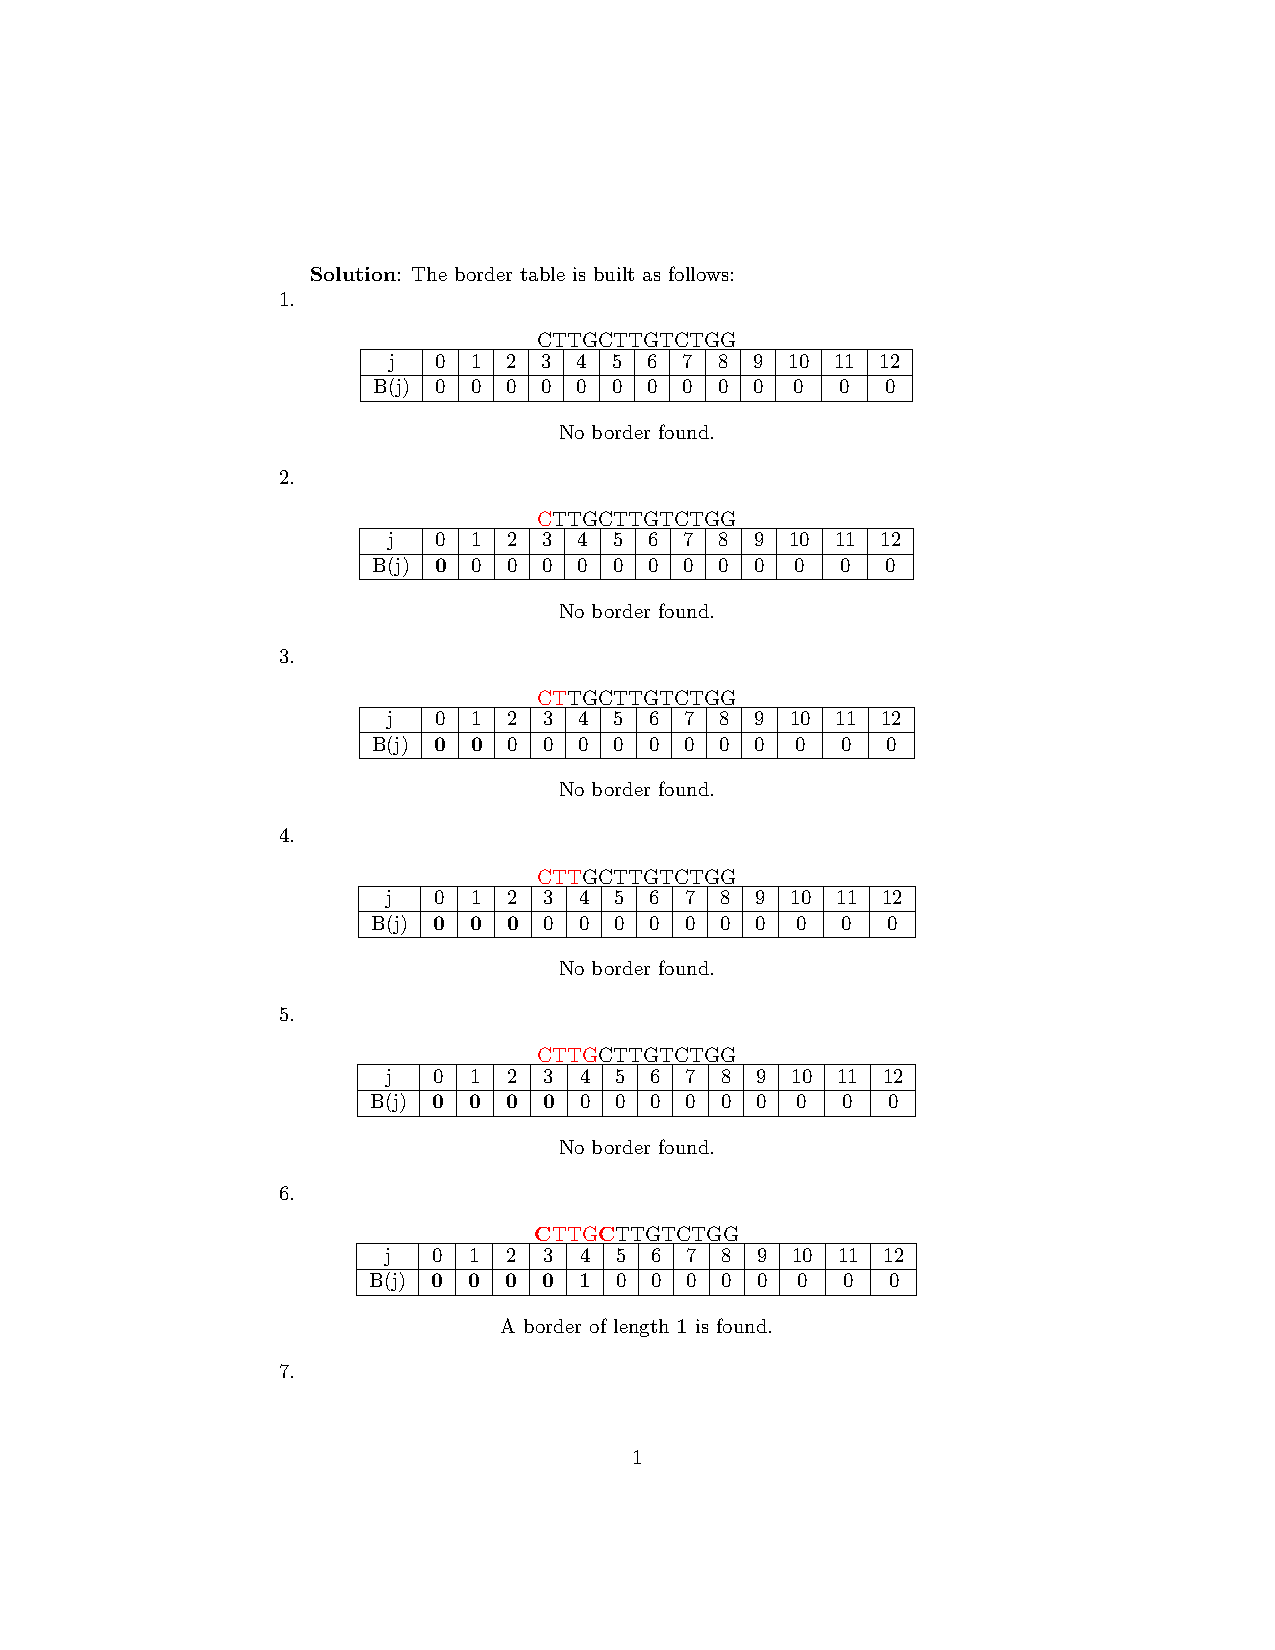
\includepdf[pages=-]{images/kmp_answer1.pdf}

\chapter{Ethics Form}
\label{chap:ethics_form}


\includepdf[pages=-]{images/ethics.pdf}

\chapter{Participant Instructions}
\label{chap:participant_instructions}

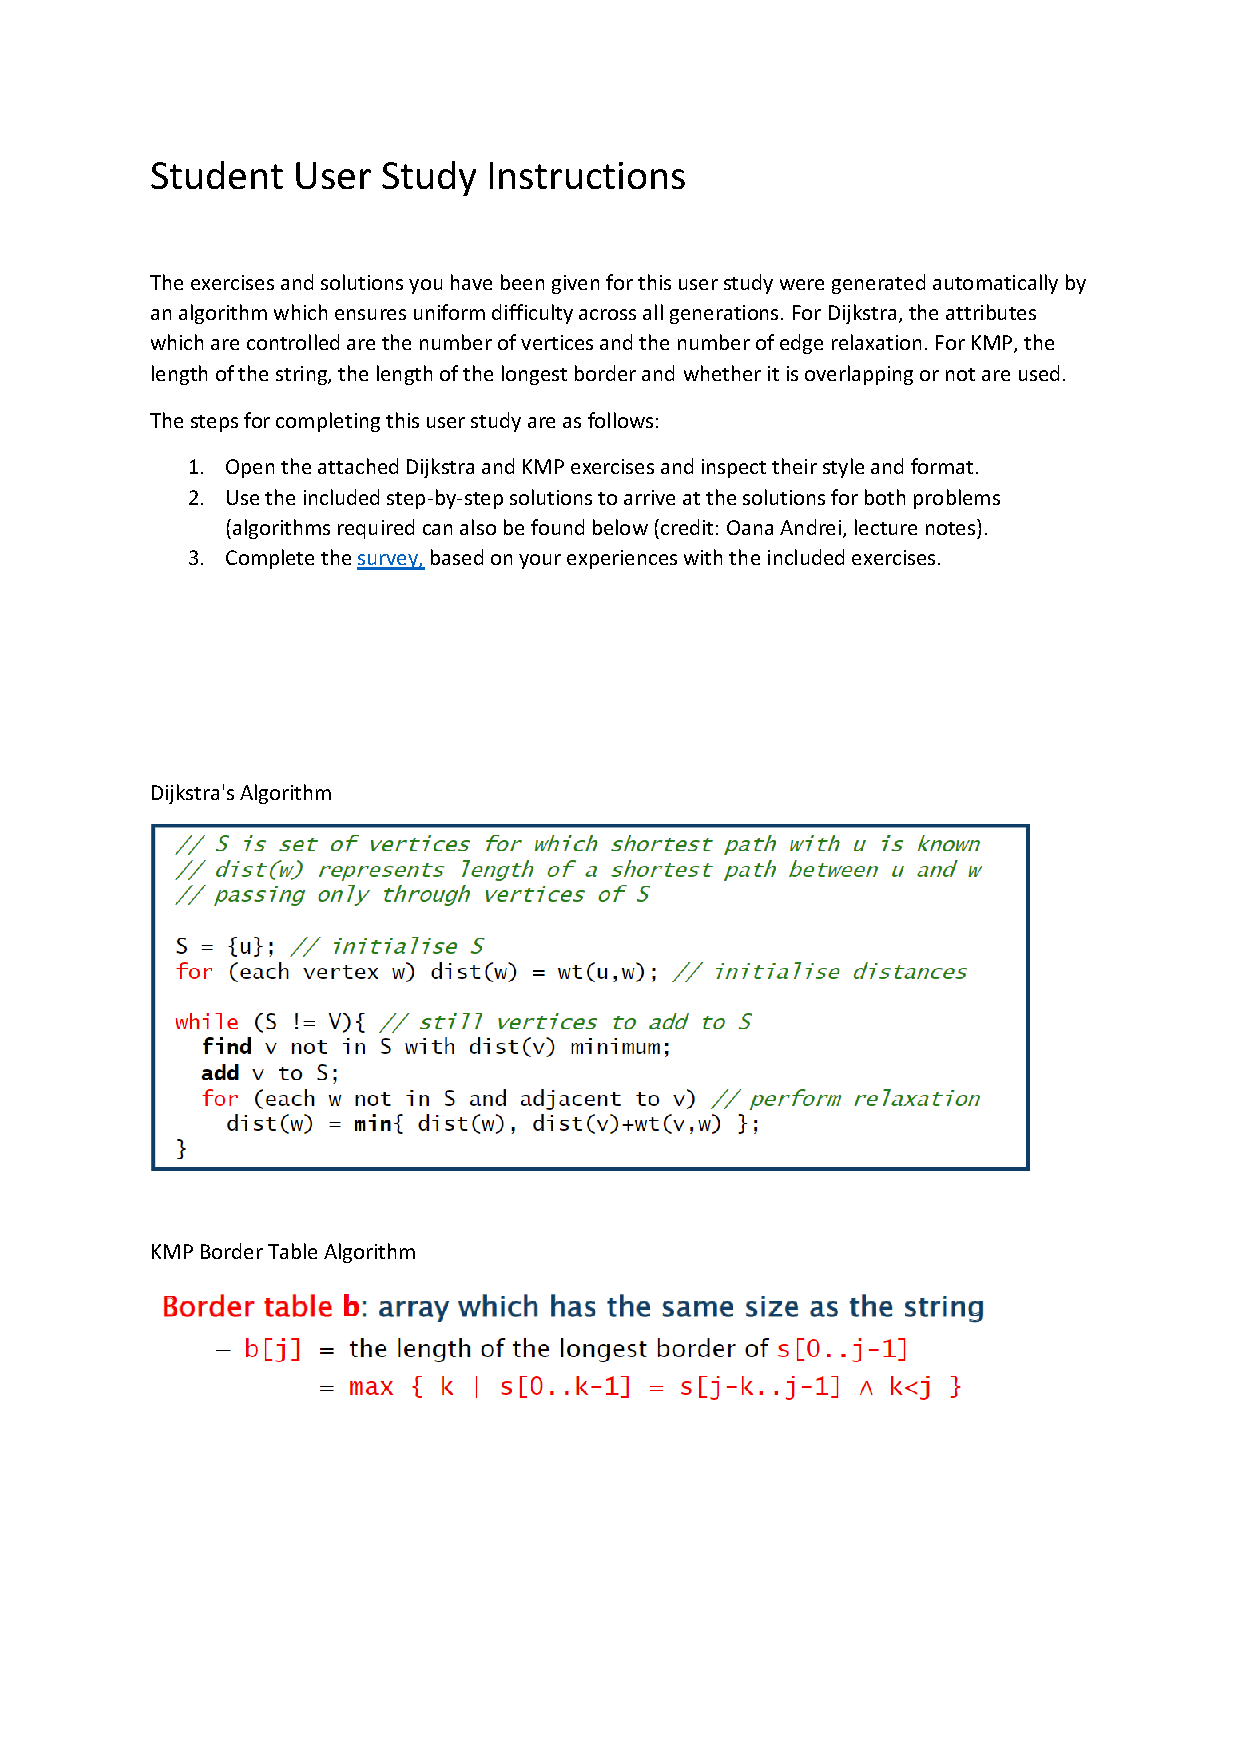
\includepdf[pages=-]{images/student_instructions.pdf}

\includepdf[pages=-]{images/lecturer_instructions.pdf}

\chapter{User surveys}
\label{chap:user_surveys}


\includepdf[pages=-]{images/student_survey.pdf}

\includepdf[pages=-]{images/lecturer_survey.pdf}

\chapter{Survey responses}
\label{sec:survey_responses}
\begin{figure}[h]
    \centering
    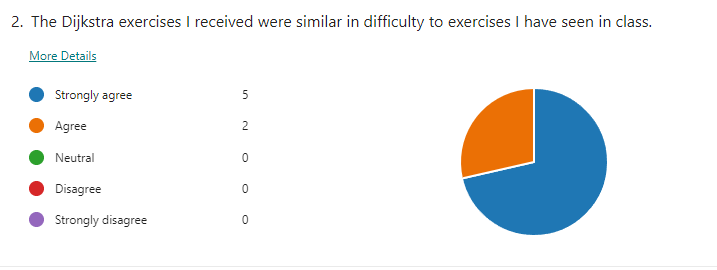
\includegraphics[width=0.9\linewidth]{images/d_similar_difficulty.png}    

    \caption{Survey responses to the question: "The Dijkstra exercises I received were similar in difficulty to exercises I have seen in class.".}
    \label{fig:d_similar_difficulty} 
\end{figure}

\begin{figure}[h]
    \centering
    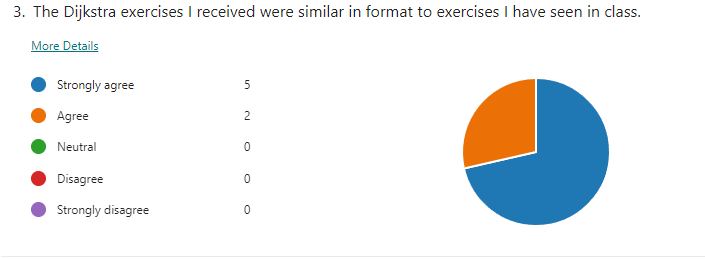
\includegraphics[width=0.9\linewidth]{images/d_similar_format.png}    

    \caption{Survey responses to the question: "The Dijkstra exercises I received were similar in format to exercises I have seen in class.".}
    \label{fig:d_similar_format} 
\end{figure}

\begin{figure}[h]
    \centering
    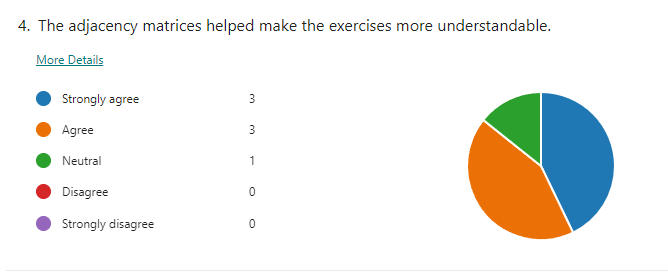
\includegraphics[width=0.9\linewidth]{images/adjacency_matrix.png}    

    \caption{Survey responses to the question: "The adjacency matrices helped make the exercises more understandable.".}
    \label{fig:adjacency_matrix} 
\end{figure}

\begin{figure}[h]
    \centering
    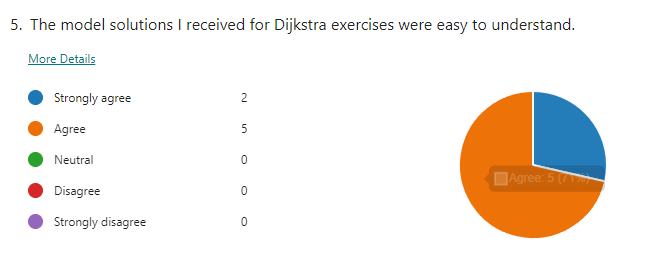
\includegraphics[width=0.9\linewidth]{images/d_model_solution.png}    

    \caption{Survey responses to the question: "The model solutions I received for Dijkstra exercises were easy to understand.".}
    \label{fig:d_model_solution} 
\end{figure}

\begin{figure}[h]
    \centering
    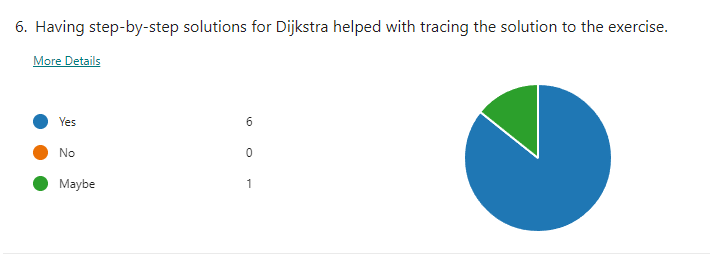
\includegraphics[width=0.9\linewidth]{images/d_step_by_step.png}    

    \caption{Survey responses to the question: "Having step-by-step solutions for Dijkstra helped with tracing the solution to the exercise.".}
    \label{fig:d_step_by_step} 
\end{figure}

\begin{figure}[h]
    \centering
    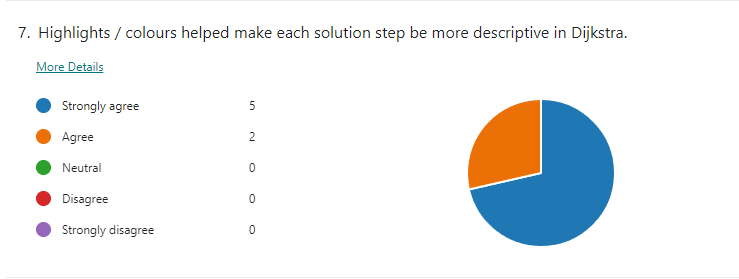
\includegraphics[width=0.9\linewidth]{images/d_highlights.png}    

    \caption{Survey responses to the question: "Highlights / colours helped make each solution step be more descriptive in Dijkstra.".}
    \label{fig:d_highlights} 
\end{figure}

\begin{figure}[h]
    \centering
    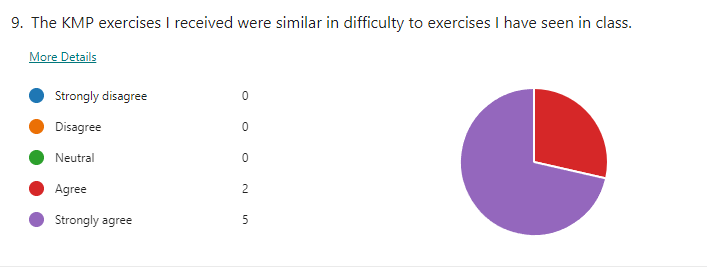
\includegraphics[width=0.9\linewidth]{images/k_similar_difficulty.png}    

    \caption{Survey responses to the question: "The KMP exercises I received were similar in difficulty to exercises I have seen in class.".}
    \label{fig:k_similar_difficulty} 
\end{figure}

\begin{figure}[h]
    \centering
    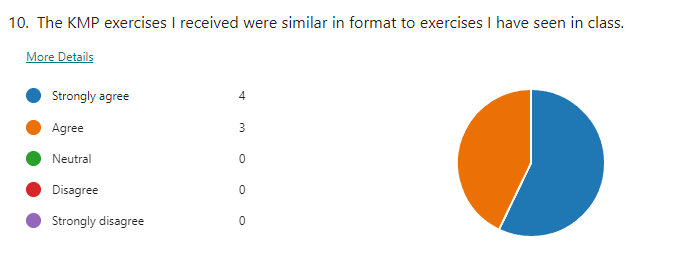
\includegraphics[width=0.9\linewidth]{images/k_similar_format.png}    

    \caption{Survey responses to the question: "The KMP exercises I received were similar in format to exercises I have seen in class.".}
    \label{fig:k_similar_format} 
\end{figure}

\begin{figure}[h]
    \centering
    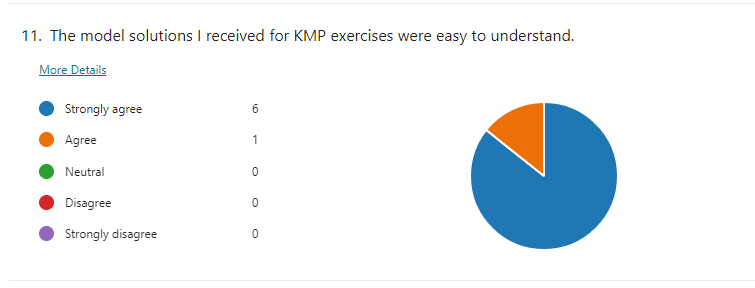
\includegraphics[width=0.9\linewidth]{images/k_model_solution.png}    

    \caption{Survey responses to the question: "The model solutions I received for KMP exercises were easy to understand.".}
    \label{fig:k_model_solution} 
\end{figure}

\begin{figure}[h]
    \centering
    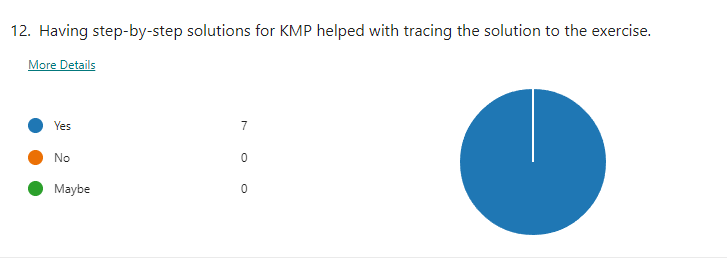
\includegraphics[width=0.9\linewidth]{images/k_step_by_step.png}    

    \caption{Survey responses to the question: "Having step-by-step solutions for KMP helped with tracing the solution to the exercise.".}
    \label{fig:k_step_by_step} 
\end{figure}

\begin{figure}[h]
    \centering
    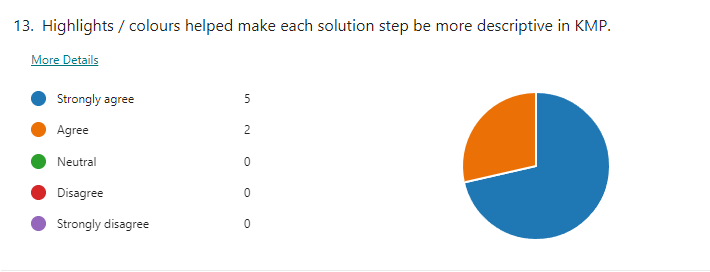
\includegraphics[width=0.9\linewidth]{images/k_highlights.png}    

    \caption{Survey responses to the question: "Highlights / colours helped make each solution step be more descriptive in KMP.".}
    \label{fig:k_highlights} 
\end{figure}

\begin{figure}[h]
    \centering
    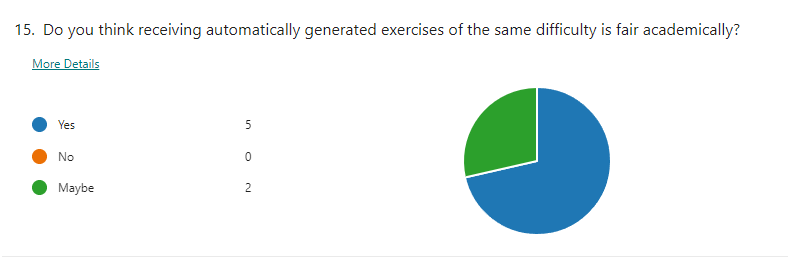
\includegraphics[width=0.9\linewidth]{images/s_academic_fair.png}    

    \caption{Survey responses to the question: "Do you think receiving automatically generated exercises of the same difficulty is fair academically?".}
    \label{fig:s_academic_fair} 
\end{figure}

\begin{figure}[h]
    \centering
    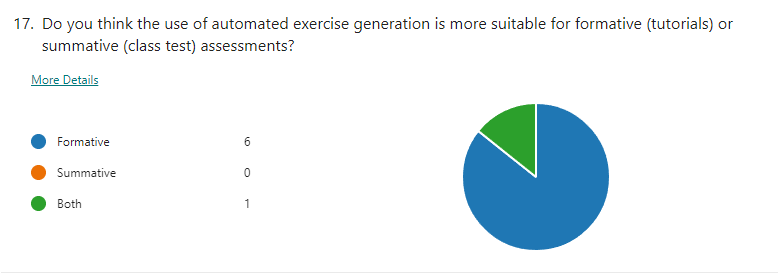
\includegraphics[width=0.9\linewidth]{images/s_formative_summative.png}    

    \caption{Survey (student) responses to the question: "Do you think the use of automated exercise generation is more suitable for formative (tutorials) or summative (class test) assessments?".}
    \label{fig:s_formative_summative} 
\end{figure}

\begin{figure}[h]
    \centering
    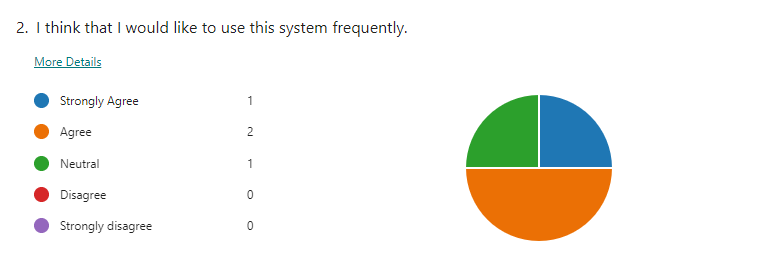
\includegraphics[width=0.9\linewidth]{images/usability1.png}    

    \caption{Survey responses to the question: "I think that I would like to use this system frequently.".}
    \label{fig:usability1} 
\end{figure}

\begin{figure}[h]
    \centering
    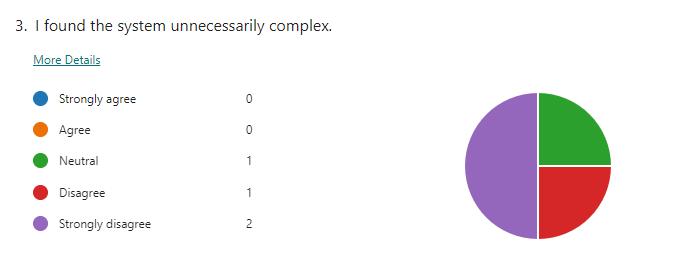
\includegraphics[width=0.9\linewidth]{images/usability2.png}    

    \caption{Survey responses to the question: "I found the system unnecessarily complex.".}
    \label{fig:usability2} 
\end{figure}

\begin{figure}[h]
    \centering
    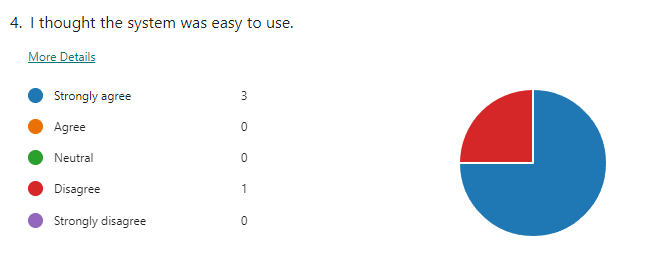
\includegraphics[width=0.9\linewidth]{images/usability3.png}    

    \caption{Survey responses to the question: "I thought the system was easy to use.".}
    \label{fig:usability3} 
\end{figure}

\begin{figure}[h]
    \centering
    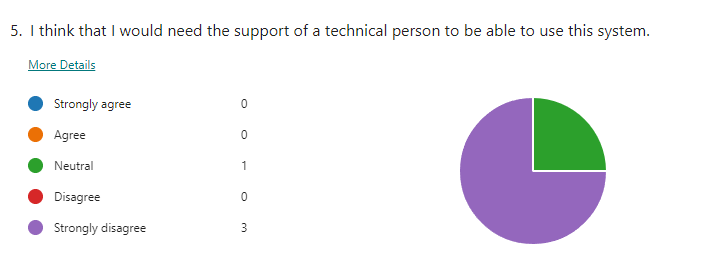
\includegraphics[width=0.9\linewidth]{images/usability4.png}    

    \caption{Survey responses to the question: "I think that I would need the support of a technical person to be able to use this system.".}
    \label{fig:usability4} 
\end{figure}

\begin{figure}[h]
    \centering
    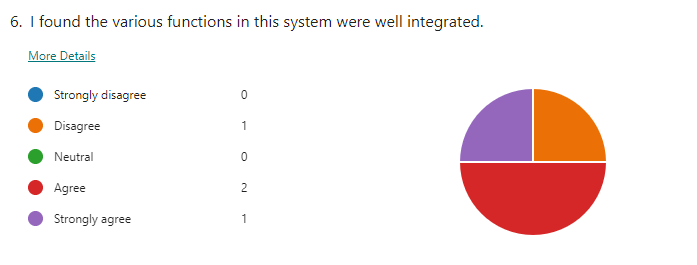
\includegraphics[width=0.9\linewidth]{images/usability5.png}    

    \caption{Survey responses to the question: "I found the various functions in this system were well integrated.".}
    \label{fig:usability5} 
\end{figure}

\begin{figure}[h]
    \centering
    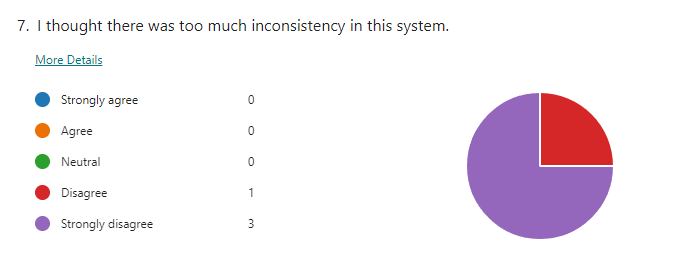
\includegraphics[width=0.9\linewidth]{images/usability6.png}    

    \caption{Survey responses to the question: "I thought there was too much inconsistency in this system.".}
    \label{fig:usability6} 
\end{figure}

\begin{figure}[h]
    \centering
    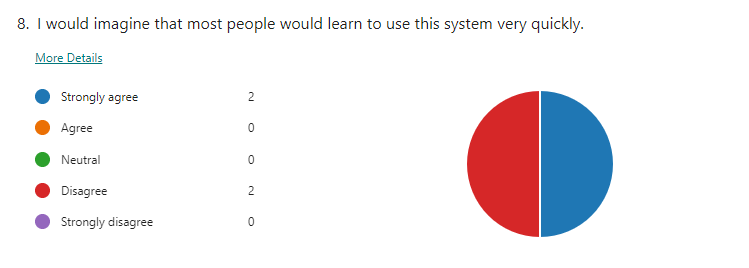
\includegraphics[width=0.9\linewidth]{images/usability7.png}    

    \caption{Survey responses to the question: "I would imagine that most people would learn to use this system very quickly.".}
    \label{fig:usability7} 
\end{figure}

\begin{figure}[h]
    \centering
    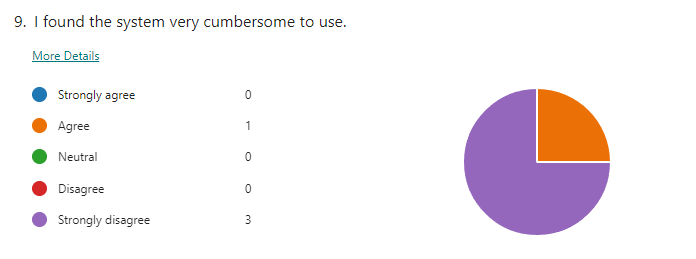
\includegraphics[width=0.9\linewidth]{images/usability8.png}    

    \caption{Survey responses to the question: "I found the system very cumbersome to use.".}
    \label{fig:usability8} 
\end{figure}

\begin{figure}[h]
    \centering
    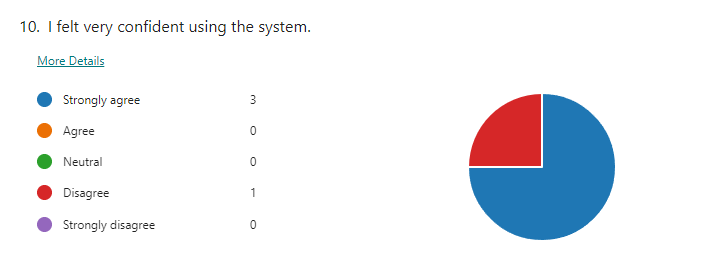
\includegraphics[width=0.9\linewidth]{images/usability9.png}    

    \caption{Survey responses to the question: "I felt very confident using the system.".}
    \label{fig:usability9} 
\end{figure}

\begin{figure}[h]
    \centering
    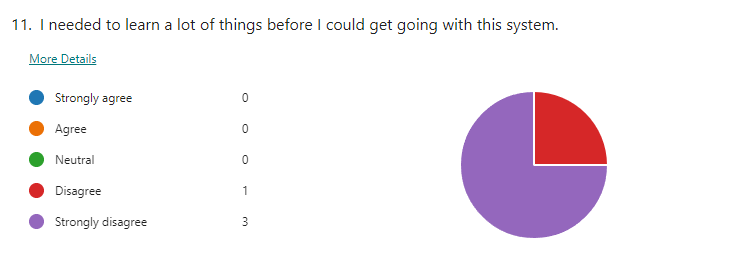
\includegraphics[width=0.9\linewidth]{images/usability10.png}    

    \caption{Survey responses to the question: "I needed to learn a lot of things before I could get going with this system.".}
    \label{fig:usability10} 
\end{figure}

\begin{figure}[h]
    \centering
    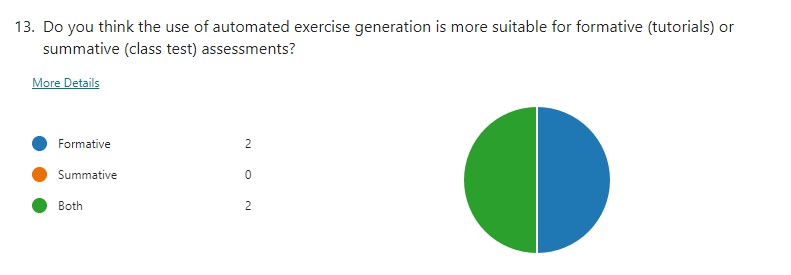
\includegraphics[width=0.9\linewidth]{images/t_summative_formative.png}    

    \caption{Survey (teacher) responses to the question: "Do you think the use of automated exercise generation is more suitable for formative (tutorials) or summative (class test) assessments?".}
    \label{fig:t_summative_formative} 
\end{figure}
\end{appendices}

%==================================================================================================================================
%   BIBLIOGRAPHY   

% The bibliography style is abbrvnat
% The bibliography always appears last, after the appendices.

\bibliographystyle{abbrvnat}

\bibliography{l4proj}

\end{document}
